\documentclass[10pt, aspectratio=169]{beamer}

% --- Configuración de Idioma y Fuentes ---
\usepackage[utf8]{inputenc}
\usepackage[spanish]{babel}
\usepackage[T1]{fontenc}
\usepackage{helvet} 

% --- Paquetes Adicionales ---
\usepackage{graphicx}
% \usepackage[space]{grffile} 
\usepackage{booktabs}
\usepackage{tikz}
\usetikzlibrary{positioning}
\usepackage{xcolor}
\usepackage{amsmath}
\usepackage{amssymb}
\usepackage{appendixnumberbeamer}
\usepackage{multirow}
\usepackage{bookmark}

% --- Rutas de imágenes ---
\graphicspath{{../../results/figures/analysis/}{../../data/processed/cis/barómetro/}}

% --- Definición de Colores IPA27 ---
\definecolor{brandgreen}{HTML}{007932}
\definecolor{softgreen}{HTML}{E8F5E9}
\definecolor{darkgrey}{HTML}{333333}
\definecolor{lightgrey}{HTML}{F5F5F5}
\definecolor{accentblue}{HTML}{0277BD}

% --- Estilo de Beamer Personalizado ---
\usetheme{Boadilla}
\usecolortheme{default}
\setbeamertemplate{navigation symbols}{} 
\setbeamertemplate{items}[circle]        
\setbeamertemplate{sections/subsections in toc}[circle]

% Arreglo de colores
\setbeamercolor{palette primary}{bg=brandgreen, fg=white}
\setbeamercolor{palette secondary}{bg=brandgreen!80, fg=white}
\setbeamercolor{palette tertiary}{bg=brandgreen!60, fg=white}
\setbeamercolor{structure}{fg=brandgreen}
\setbeamercolor{title}{fg=brandgreen, bg=white}
\setbeamercolor{frametitle}{fg=brandgreen, bg=white}
\setbeamercolor{block title}{bg=brandgreen, fg=white}
\setbeamercolor{block body}{bg=softgreen, fg=black}

% Ajuste de pie de página
% Ajuste de pie de página simplificado
\setbeamertemplate{footline}{
  \leavevmode%
  \hbox{%
  \begin{beamercolorbox}[wd=.3333\paperwidth, left]{author in head/foot}%
    \hspace*{2ex}IPA27 Project - Metodología Detallada
  \end{beamercolorbox}%
  \begin{beamercolorbox}[wd=.3333\paperwidth, center]{title in head/foot}%
    \insertshorttitle
  \end{beamercolorbox}%
  \begin{beamercolorbox}[wd=.3333\paperwidth, right]{date in head/foot}%
    \insertframenumber{} / \inserttotalframenumber\hspace*{2ex} 
  \end{beamercolorbox}}%
  \vskip0pt%
}

% --- Configuración del Logotipo Corporativo ---
\logo{
\includegraphics[width=1cm,keepaspectratio]{logo_fa27.png}}

% --- Información de Portada ---
\title[IPA27: Análisis de Prosperidad]{Índice de Prosperidad Andaluz (IPA27)}
\subtitle{Arquitectura Técnica, Metodología de Armonización y Resultados (2016-2025)}
\author[Equipo IPA27]{Fundación Andalucía 27}
\date{\today}

\begin{document}

% --- Slide de Título Premium ---
{
\setbeamertemplate{footline}{} 
\begin{frame}[plain]
    \begin{tikzpicture}[remember picture, overlay]
        % 1. Wide and Premium Sidebar
        \fill[brandgreen] (current page.north west) rectangle ([xshift=4.5cm]current page.south west);
        
        % 2. Prominent White Logo in Sidebar
        \node[anchor=north] at ([xshift=2.25cm, yshift=-1.5cm]current page.north west) {
            
\includegraphics[width=3cm, keepaspectratio]{logo_fa27_white.png}
        };
        
        % 4. Main Title Block on White Side
        \node[anchor=north west, xshift=5.5cm, yshift=-2.5cm] at (current page.north west) {
            \begin{minipage}{0.6\paperwidth}
                {\fontsize{64}{74}\selectfont \textbf{\textcolor{brandgreen}{IPA27}}} \\[0.3cm]
                {\fontsize{26}{32}\selectfont \textcolor{darkgrey}{Índice de Prosperidad Andaluz}} \\[1.5cm]
                {\color{brandgreen!30}\rule{8cm}{5pt}} \\[0.8cm]
                {\Large \textcolor{darkgrey}{\textbf{Arquitectura Técnica, Metodología de Armonización} \\ y Análisis de Resultados (2016-2025)}}
            \end{minipage}
        };
        
        % 5. Elegant Footer Detail
        \node[anchor=south east, xshift=-1cm, yshift=1.5cm] at (current page.south east) {
            \begin{minipage}{0.4\paperwidth}
                \raggedleft
                {\Large \textbf{\textcolor{brandgreen}{Fundación Andalucía 27}}} \\
                \vspace{0.1cm}
                \textcolor{darkgrey}{\today}
            \end{minipage}
        };
    \end{tikzpicture}
\end{frame}
}

% --- Separador de Secciones comentado ---

% --- 1. INTRODUCCIÓN ---
\section{Introducción}

{
\setbeamercolor{background canvas}{bg=brandgreen}
\begin{frame}[plain]
    \centering
    \vfill
    {\Huge\bfseries\color{white} I. INTRODUCCIÓN}\\[0.6cm]
    {\color{white}\rule{6cm}{2.5pt}}\\[1.5cm]
    
\includegraphics[width=2.5cm]{logo_fa27_white.png}
    \vfill
\end{frame}
}

\begin{frame}{Gobernanza y Rigor Técnico}
    \begin{columns}[T]
        % --- COLUMNA IZQUIERDA: Liderazgo y Propósito ---
        \begin{column}{0.38\textwidth}
            \setbeamercolor{block title}{bg=brandgreen, fg=white}
            \begin{block}{Dirección Técnica}
                \textbf{Manuel Alejandro Hidalgo} \\
                \vspace{0.1cm}
                \scriptsize Profesor de Economía Aplicada (UPO). \\
                Responsable del diseño y supervisión.
            \end{block}

            \vspace{0.6cm}

            \setbeamercolor{block title}{bg=darkgrey, fg=white}
            \begin{block}{Misión del Consejo}
                \scriptsize Garantizar la independencia, el rigor estadístico y la excelencia académica en el IPA27.
            \end{block}
        \end{column}

        % --- COLUMNA DERECHA: Lista de Expertos ---
        \begin{column}{0.58\textwidth}
            \textbf{\textcolor{brandgreen}{Consejo Técnico Asesor}}
            \vspace{0.3cm}
            
            % Usamos un entorno de descripción personalizado para mayor claridad
            \begin{description}[font=\bfseries\color{brandgreen}\small]
                \item[Rafael Doménech] \scriptsize BBVA Research / Univ. de Valencia.
                \item[Olga Cantó] \scriptsize Universidad de Alcalá.
                \item[Antonio Villar] \scriptsize IVIE / Universidad Pablo de Olavide.
                \item[Miguel Ángel García] \scriptsize Universidad Rey Juan Carlos.
                \item[Lucía Gorjón] \scriptsize Fundación ISEAK.
            \end{description}
            
            \vspace{0.4cm}
            \begin{tikzpicture}
                \fill[lightgrey] (0,0) rectangle (\textwidth, 0.02);
            \end{tikzpicture}
        \end{column}
    \end{columns}
\end{frame}

\begin{frame}{El paradigma de la Prosperidad en el Siglo XXI}
    \begin{columns}
        \begin{column}{0.6\textwidth}
            \textbf{Más allá del PIB: El consenso internacional}
            \begin{itemize}
                \item \textit{Informe Stiglitz-Sen-Fitoussi (2009)}: Necesidad de medir el bienestar real y la sostenibilidad.
                \item \textbf{Alineación con los ODS}: No dejar a nadie atrás.
            \end{itemize}
            \vspace{0.4cm}
            \textbf{Misión del IPA27}
            \begin{itemize}
                \item Medir el progreso sistémico de Andalucía.
                \item Proporcionar una herramienta de \textbf{monitorización trimestral} (no anual).
                \item Comparar frente al conjunto nacional y el resto de regiones españolas (CC.AA.).
            \end{itemize}
        \end{column}
        \begin{column}{0.4\textwidth}
            \begin{block}{Definición de Prosperidad}
                No es solo acumulación de capital, sino la capacidad de una sociedad de ofrecer a sus ciudadanos seguridad, libertad y oportunidades vitales.
            \end{block}
        \end{column}
    \end{columns}
\end{frame}

% --- 2. ARQUITECTURA DETALLADA ---
\section{Arquitectura}

{
\setbeamercolor{background canvas}{bg=brandgreen}
\begin{frame}[plain]
    \centering
    \vfill
    {\Huge\bfseries\color{white} II. ARQUITECTURA}\\[0.6cm]
    {\color{white}\rule{6cm}{2.5pt}}\\[1.5cm]
    
\includegraphics[width=2.5cm]{logo_fa27_white.png}
    \vfill
\end{frame}
}

\begin{frame}{Estructura Jerárquica: Los 3 Dominios}
    \centering
    \begin{tikzpicture}[node distance=1.2cm and 1cm, every node/.style={fill=white, font=\sffamily}, 
                        block/.style={draw=darkgrey, thick, rounded corners, align=center, inner sep=5pt, text width=3.8cm}]
        \node (ipa) [draw=brandgreen, ultra thick, rounded corners, fill=softgreen, inner sep=10pt] {\huge \textbf{IPA27}};
        
        \node (d2) [block, below = 1.2cm of ipa] {\textbf{Economías Abiertas}\\ \footnotesize (4 Pilares / 8 Ind.)};
        \node (d1) [block, left = of d2] {\textbf{Sociedades Inclusivas}\\ \footnotesize (4 Pilares / 8 Ind.)};
        \node (d3) [block, right = of d2] {\textbf{Personas Empoderadas}\\ \footnotesize (4 Pilares / 8 Ind.)};
        
        \coordinate (below_ipa) at ([yshift=-0.6cm]ipa.south);
        
        \draw[brandgreen, ultra thick] (ipa.south) -- (below_ipa);
        \draw[->, brandgreen, ultra thick] (below_ipa) -| (d1.north);
        \draw[->, brandgreen, ultra thick] (below_ipa) -- (d2.north);
        \draw[->, brandgreen, ultra thick] (below_ipa) -| (d3.north);
    \end{tikzpicture}
    
    \vspace{0.5cm}
    \begin{itemize}
        \item \textbf{Sociedades Inclusivas}: Calidad del entorno cívico e institucional.
        \item \textbf{Economías Abiertas}: Capacidad productiva, infraestructura y competitividad.
        \item \textbf{Personas Empoderadas}: Desarrollo humano, educación y bienestar.
    \end{itemize}
\end{frame}

\begin{frame}{Dominio 1: Sociedades Inclusivas}
    \begin{table}
        \centering
        \footnotesize
        \begin{tabular}{llp{7cm}}
            \toprule
            \textbf{Pilar} & \textbf{Indicador} & \textbf{Concepto} \\
            \midrule
            \multirow{2}{*}{1. Seguridad} & SEG\_BAL & Balance de Criminalidad (Hurtos + Robos). \\
             & SEG\_CRI & Tasa de Criminalidad Total por 100k hab. \\
            \midrule
            \multirow{2}{*}{2. Libertad} & LIB\_ODI & Delitos de Odio (cohesión y convivencia). \\
             & LIB\_SEX & Libertad Sexual e Indemnidad. \\
            \midrule
            \multirow{2}{*}{3. Gobernanza} & GOB\_DES & Índice de Desafección Política (CIS). \\
             & GOB\_EFF & Eficiencia Judicial frente a la Corrupción. \\
            \midrule
            \multirow{2}{*}{4. Capital Social} & SOC\_ASO & Afiliados a Actividades Asociativas. \\
             & SOC\_PAR\_enlazado & Participación Electoral (procesos enlazados). \\
            \bottomrule
        \end{tabular}
    \end{table}
\end{frame}

\begin{frame}{Dominio 2: Economías Abiertas}
    \begin{table}
        \centering
        \footnotesize
        \begin{tabular}{llp{7cm}}
            \toprule
            \textbf{Pilar} & \textbf{Indicador} & \textbf{Concepto} \\
            \midrule
            \multirow{2}{*}{5. Inversión} & INV\_HIP & Constitución de Hipotecas (Dinamismo Mercantil). \\
             & INV\_IED & Inversión Extranjera Directa (\% sobre PIB). \\
            \midrule
            \multirow{2}{*}{6. Empresas} & EMP\_NAT & Natalidad Empresarial (Empresas creadas). \\
             & EMP\_SOC & Constitución de Sociedades Mercantiles. \\
            \midrule
            \multirow{2}{*}{7. Infraestructura} & INF\_BAN & Penetración de Banda Ancha y Conectividad. \\
             & INF\_TRA & Uso del Transporte Público (Viajeros). \\
            \midrule
            \multirow{2}{*}{8. Calidad Económica} & ECO\_RBHpc & Renta Bruta de los Hogares per cápita (Real). \\
             & ECO\_COL\_sal & Coste Salarial Ordinario (por trabajador). \\
            \bottomrule
        \end{tabular}
    \end{table}
\end{frame}

\begin{frame}{Dominio 3: Personas Empoderadas}
    \begin{table}
        \centering
        \footnotesize
        \begin{tabular}{llp{7cm}}
            \toprule
            \textbf{Pilar} & \textbf{Indicador} & \textbf{Concepto} \\
            \midrule
            \multirow{2}{*}{9. Vida} & VID\_ARO & Tasa AROPE (Riesgo de Pobreza o Exclusión). \\
             & VID\_PAR & Tasa de Paro (Inverso: Tasa de Empleo EPA). \\
            \midrule
            \multirow{2}{*}{10. Salud} & SAL\_ESP & Esperanza de Vida al Nacer. \\
             & SAL\_SAT\_enlazado & Satisfacción con el Sistema Sanitario Público. \\
            \midrule
            \multirow{2}{*}{11. Educación} & EDU\_ABA & Tasa de Abandono Escolar Temprano. \\
             & EDU\_SUP & Población con Educación Superior (Nivel Competencial). \\
            \midrule
            \multirow{2}{*}{12. Conocimiento} & CON\_IDI & Inversión en I+D (\% del PIB). \\
             & CON\_OCI & Afiliados en Sectores de Conocimiento (OCI). \\
            \bottomrule
        \end{tabular}
    \end{table}
\end{frame}

% --- 3. METODOLOGÍA: DESARROLLO TÉCNICO ---
\section{Metodología}

{
\setbeamercolor{background canvas}{bg=brandgreen}
\begin{frame}[plain]
    \centering
    \vfill
    {\Huge\bfseries\color{white} III. METODOLOGÍA}\\[0.6cm]
    {\color{white}\rule{6cm}{2.5pt}}\\[1.5cm]
    
\includegraphics[width=2.5cm]{logo_fa27_white.png}
    \vfill
\end{frame}
}

\begin{frame}{Fuentes y Automatización de Datos}
    \begin{columns}[T]
        \begin{column}{0.45\textwidth}
            \textbf{El Diccionario Maestro (\textit{Master Dictionary})}
            \begin{itemize}
                \item Repositorio único de metadatos.
                \item Parámetros de filtrado y transformación.
            \end{itemize}
            \vspace{0.3cm}
            \textbf{Conectores Automáticos}
            \begin{itemize}
                \item \textbf{INE / IECA}: APIs REST (Tempus/JAXI).
                \item \textbf{Scraping}: Balances de criminalidad.
                \item \textbf{Carga}: Inversión Extranjera (MINECO).
            \end{itemize}
        \end{column}
        \begin{column}{0.55\textwidth}
            \centering
            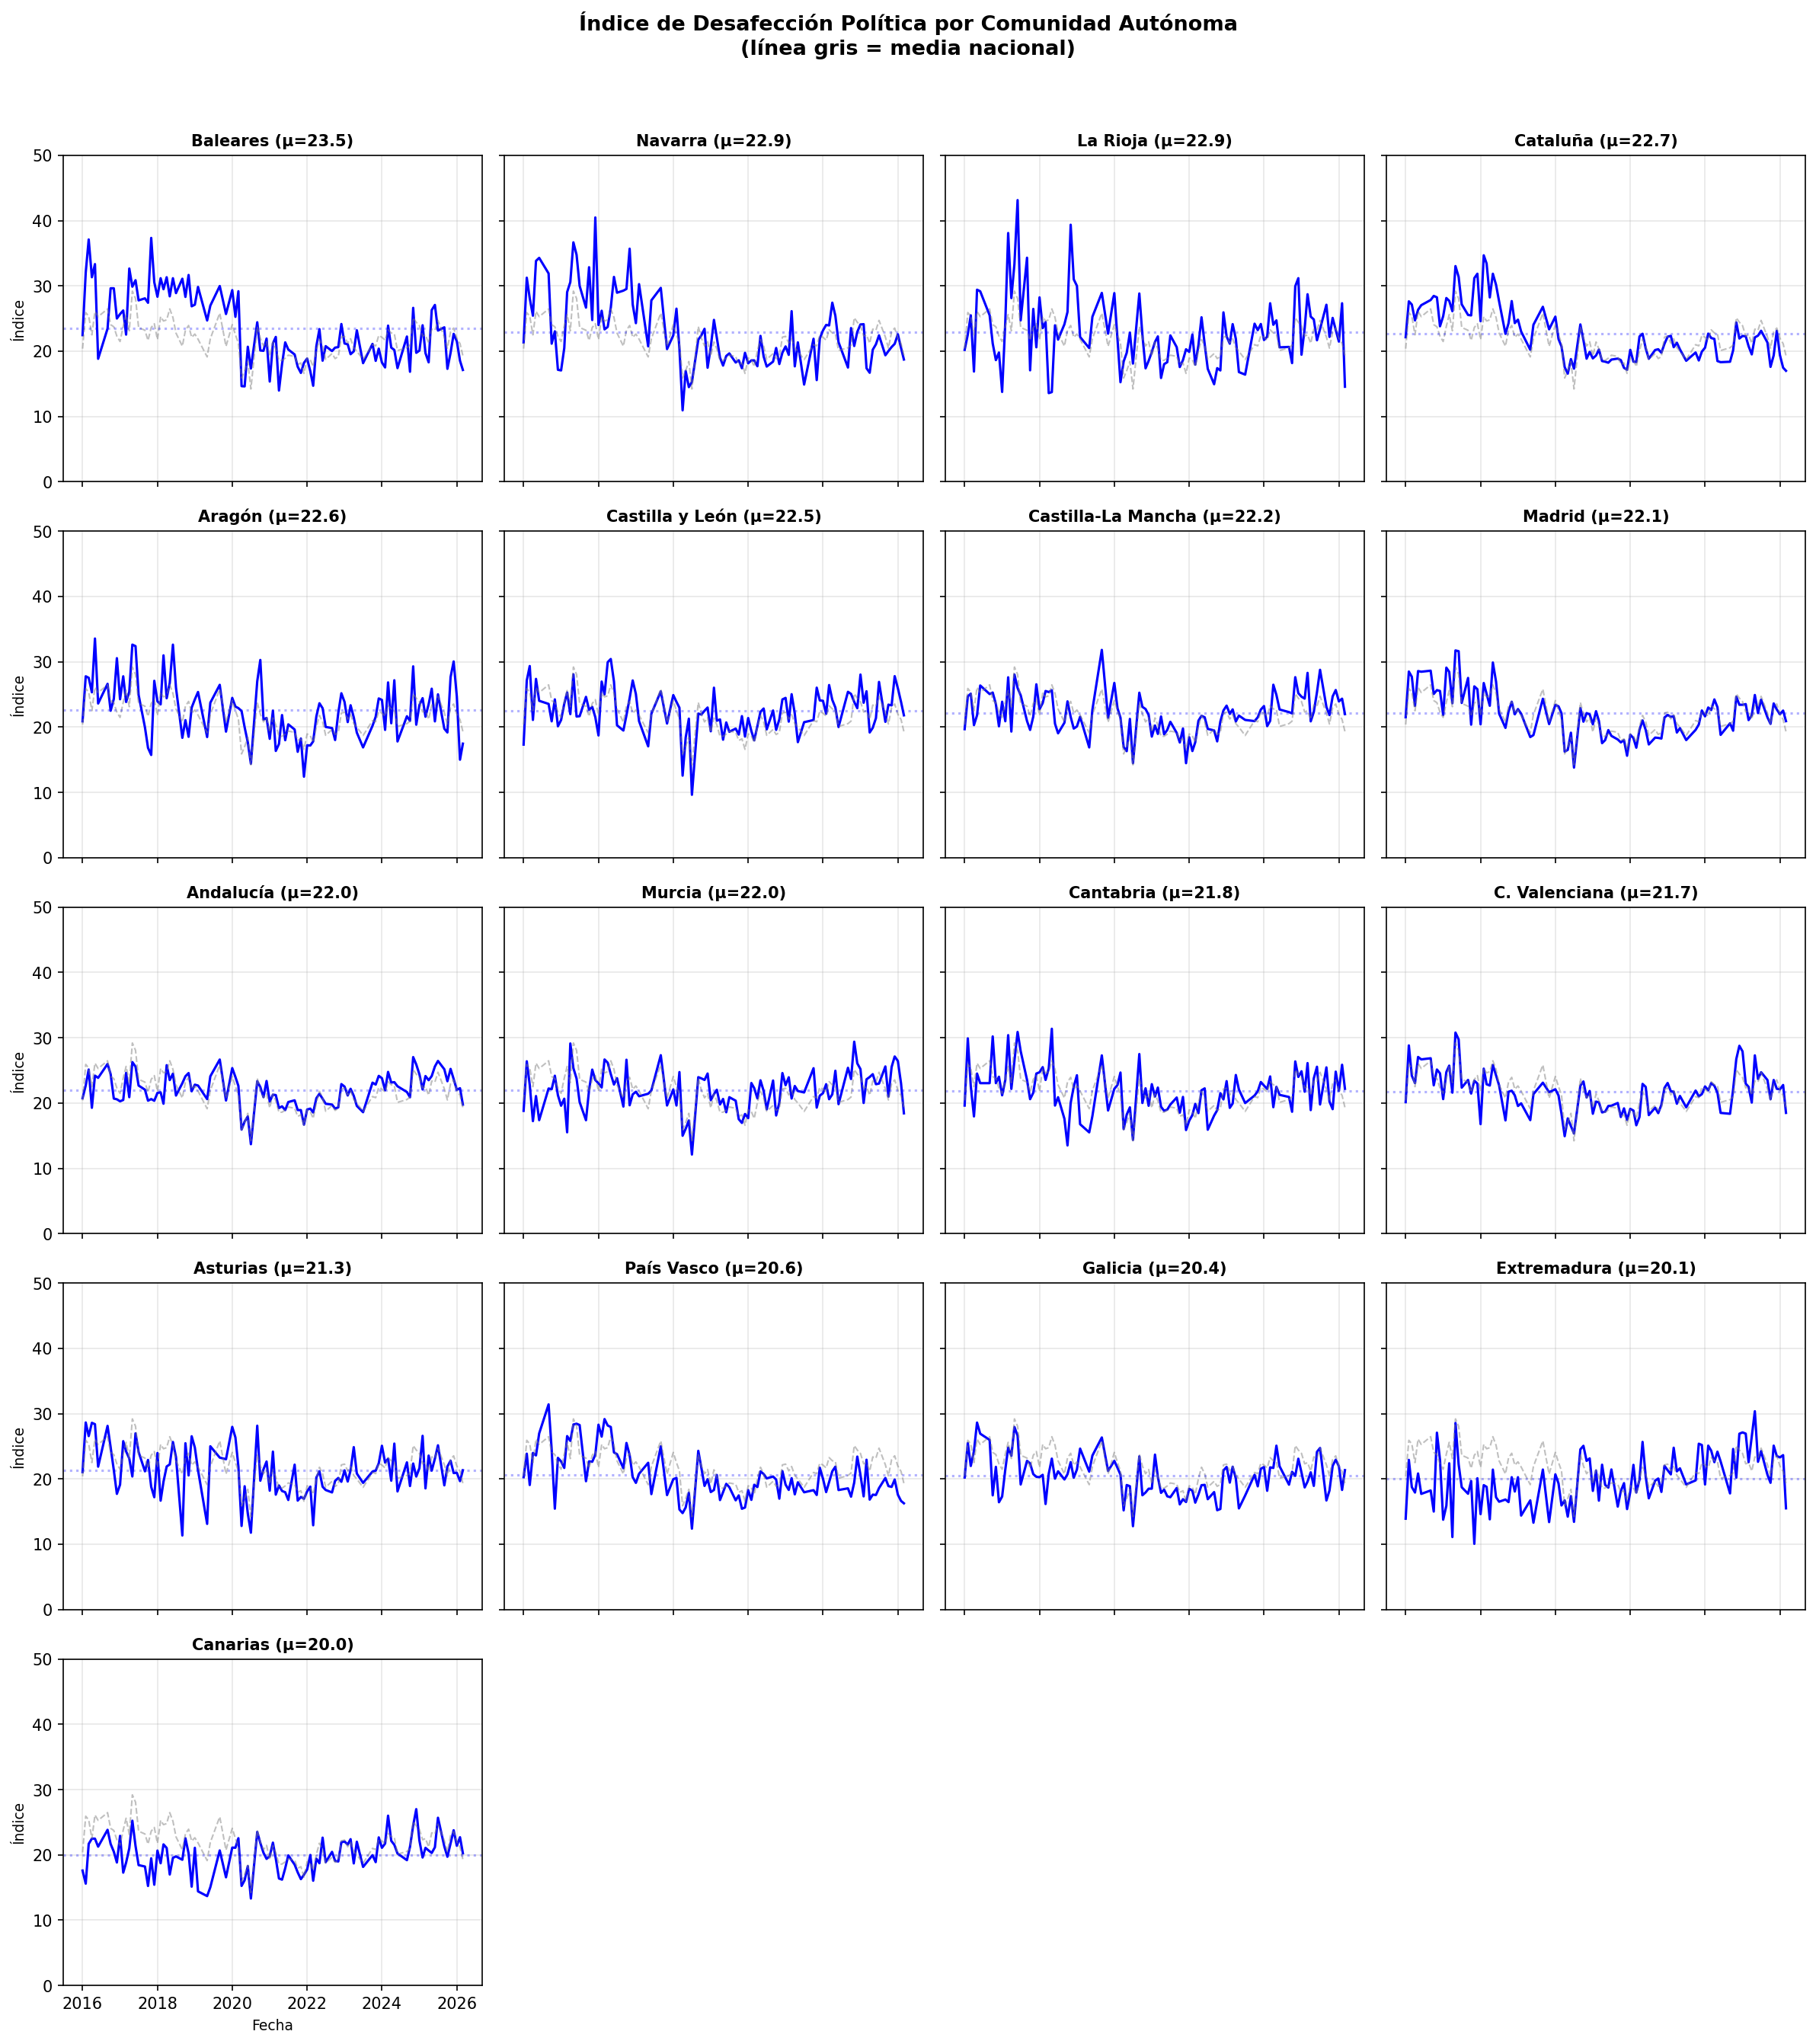
\includegraphics[width=0.8\textwidth]{desafeccion_por_ccaa.png} \\
            \tiny \textit{Ejemplo: Procesamiento de microdatos del CIS (Gobernanza).}
        \end{column}
    \end{columns}
    \begin{block}{Trazabilidad Total y Auditoría}
        Cada observación cuenta con un \textit{vintage} fechado, permitiendo reconstruir y auditar cualquier punto histórico del índice desde el dato bruto oficial.
    \end{block}
\end{frame}

\begin{frame}{Tratamiento de Series Trimestrales}
    Para que el índice sea comparable, todas las series deben ser trimestrales.
    \vspace{0.4cm}
    \begin{description}
        \item[Desestacionalización (STL):] Eliminamos el ruido del calendario (Navidad, Verano) usando \textit{Seasonal-Trend decomposition using Loess} robusto.
        \item[Trimestralización (Chow-Lin):] Es el núcleo econométrico del IPA27. Convierte datos anuales (ej: I+D, AROPE) a trimestrales usando un benchmark de alta frecuencia.
        \[ y_{q} = \beta x_{q} + u_{q}, \quad u_{q} = \rho u_{q-1} + \epsilon_q \]
        \item[Nowcasting (ARIMA):] Predicción técnica del último trimestre cuando las fuentes oficiales aún no han publicado el dato (ej: 2025Q4).
    \end{description}
\end{frame}

\begin{frame}{Normalización por Techos Fijos}
    
    \textbf{¿Por qué NO usar Min-Max?}
    \begin{itemize}
        \item El score de 2018 cambiaría hoy si Madrid mejora su máximo en 2025.
        \item Es inestable para el análisis histórico.
    \end{itemize}

    \vspace{0.4cm} % Espacio estético entre bloques

    \textbf{La solución: El Techo de Excelencia}
    \begin{itemize}
        \item Calculamos un \textbf{Techo} empírico basado en las \textbf{Top 3} regiones líderes.
        \item Agregamos un horizonte de mejora proyectado a 5 años.
    \end{itemize}

    \vspace{0.3cm}

    \[ Score = \left( \frac{\text{Valor actual}}{\text{Techo Fijo}} \right) \times 100 \]

    \vspace{0.4cm}

    \begin{exampleblock}{Escala 0-120}
        Si una región supera el techo (excelencia excepcional), su score puede llegar a 120 puntos.
    \end{exampleblock}

\end{frame}

\begin{frame}{Agregación Geométrica: Complementariedad}
    \textbf{Concepto de Complementariedad}
    \begin{itemize}
        \item La prosperidad requiere equilibrio.
        \item Un 100 en Salud no compensa un 0 en Seguridad.
        \item La \textbf{Media Geométrica} penaliza los desequilibrios sectoriales.
    \end{itemize}
    \vspace{0.4cm}
    \textbf{Penalización por Desequilibrio}
    \[ \text{Penalización} = \text{Media Aritmética} - \text{Media Geométrica} \]
\end{frame}

% --- 4. RESULTADOS DETALLADOS ---
\section{Resultados}

{
\setbeamercolor{background canvas}{bg=brandgreen}
\begin{frame}[plain]
    \centering
    \vfill
    {\fontsize{50}{60}\selectfont\bfseries\color{white} IV. RESULTADOS}\\[0.8cm]
    {\color{white}\rule{8cm}{4pt}}\\[1.5cm]
    
\includegraphics[width=3cm]{logo_fa27_white.png}
    \vfill
\end{frame}
}

\begin{frame}{Evolución Temporal: Andalucía vs España (2016-2025)}
    \centering
    
\includegraphics[width=0.8\textwidth]{ipa27_evolucion_temporal.png}
    \vfill
    \begin{itemize}
        \item \textbf{Tendencia ascendente}: Crecimiento sostenido de la prosperidad desde 2016.
        \item \textbf{Brecha estructural}: Se mantiene un diferencial con la media nacional, pero con signos de convergencia en el último trienio.
    \end{itemize}
\end{frame}

\begin{frame}{Análisis de Brechas por Dominio}
    \begin{columns}
        \begin{column}{0.65\textwidth}
            \centering
            
\includegraphics[width=0.9\linewidth, keepaspectratio]{ipa27_brechas_dominios.png}
        \end{column}
        \begin{column}{0.35\textwidth}
            \textbf{Diferencial AND vs ESP}
            \begin{itemize}
                \item ¿Dónde nos alejamos del patrón nacional? 
                \item \textbf{Fortalezas}: Capital Social y Salud.
                \item \textbf{Desafíos}: Dinamismo empresarial e Innovación.
            \end{itemize}
        \end{column}
    \end{columns}
\end{frame}

\begin{frame}{Perfil por Dominios: Análisis de Radar (Media 2025)}
    \centering
    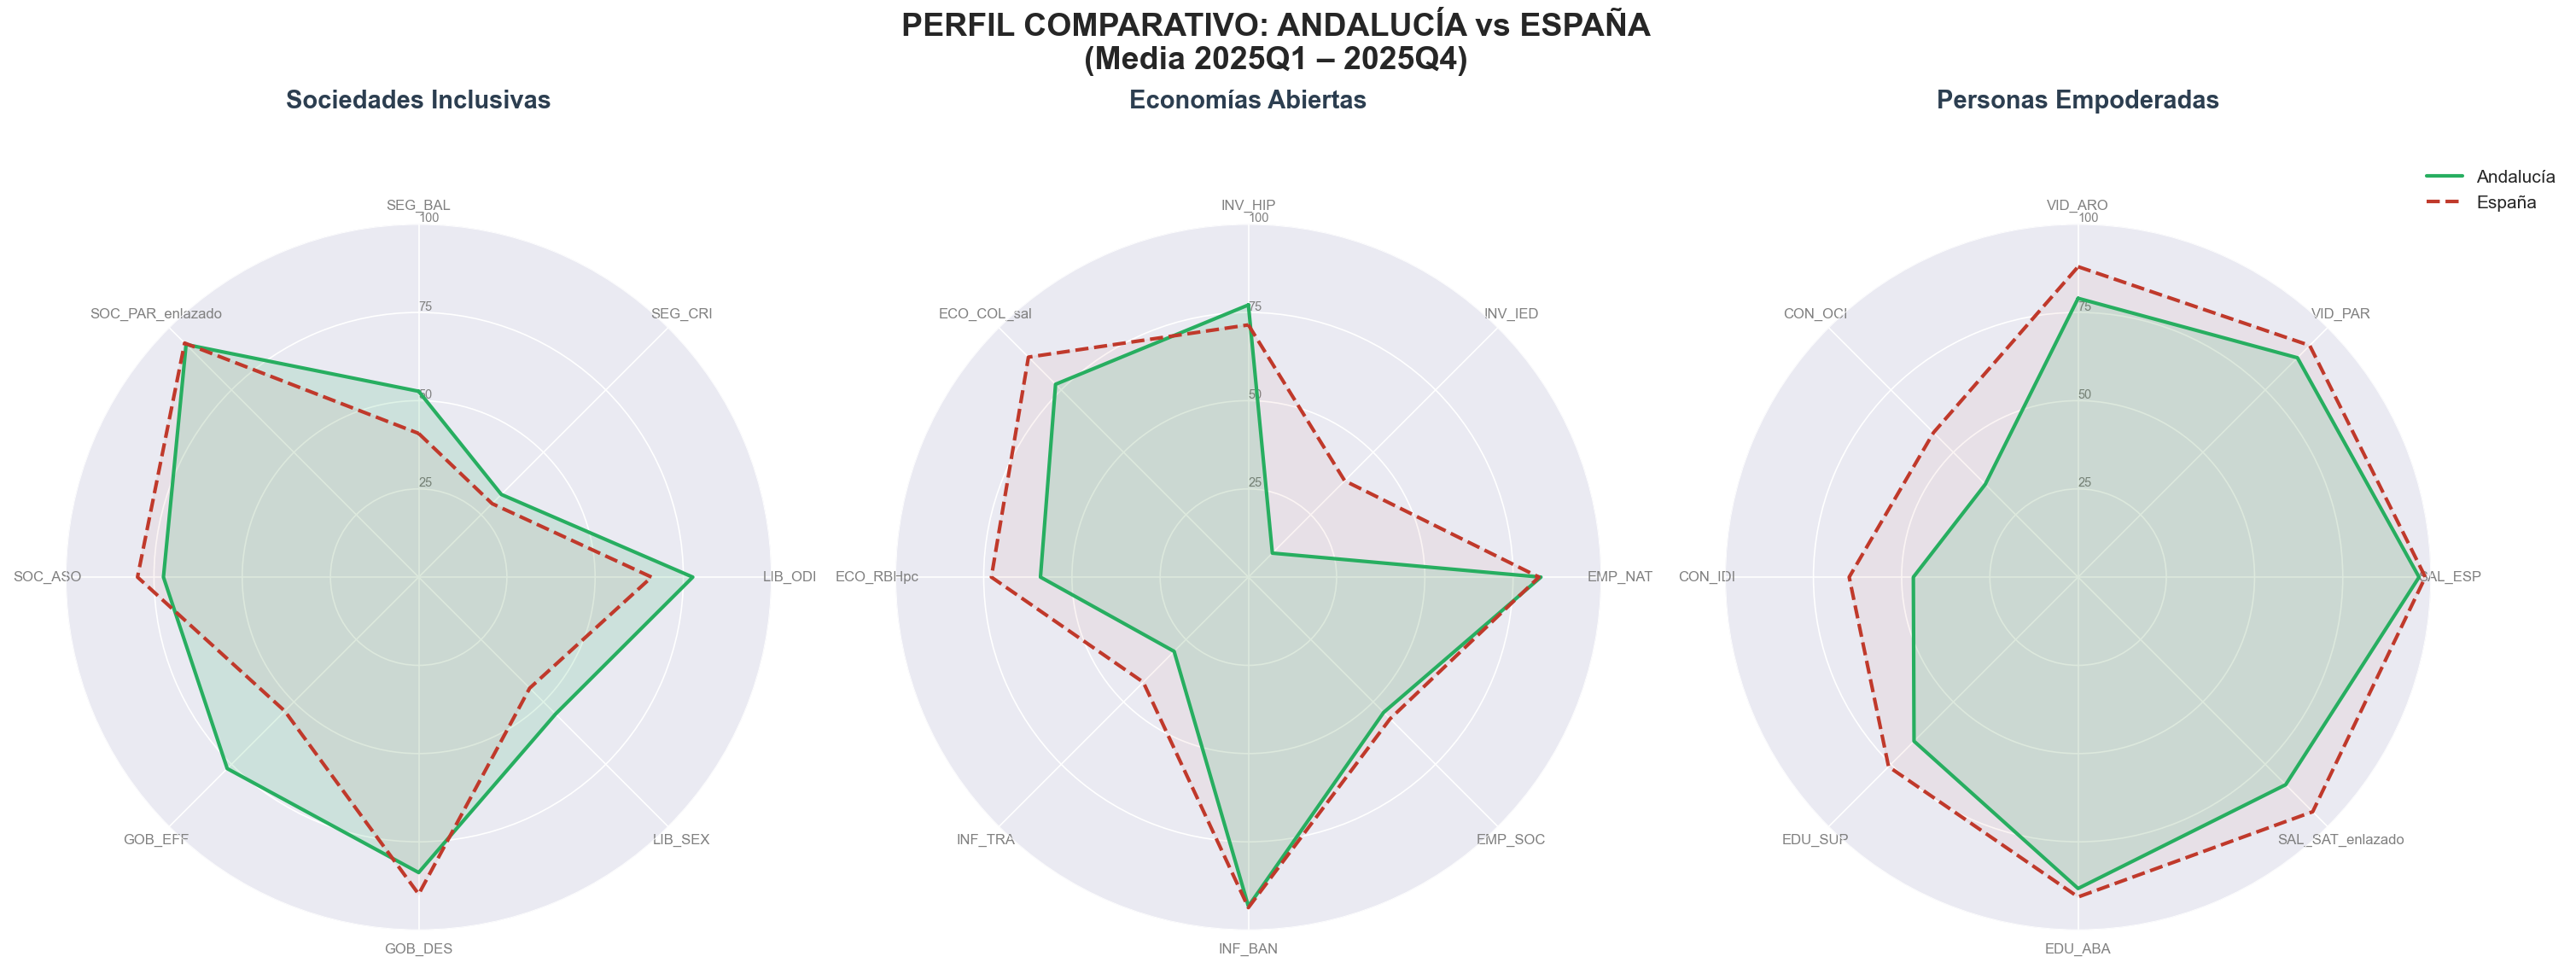
\includegraphics[width=0.8\linewidth]{radar_dominios_and_esp_media4q.png}
    \vfill
    \begin{itemize}
        \small
        \item \textbf{Sociedades Inclusivas}: Liderazgo destacado en Seguridad y Gobernanza frente a la media nacional.
        \item \textbf{Economías Abiertas}: Brecha significativa en Inversión Extranjera (IED), aunque competitiva en Mercado de Capitales.
        \item \textbf{Personas Empoderadas}: Fortaleza en Salud (Satisfacción) compensando desafíos en Educación y Conocimiento.
    \end{itemize}
\end{frame}

\begin{frame}{Vectores de Avance: Top y Bottom Indicadores (2023-2025)}
    \centering
    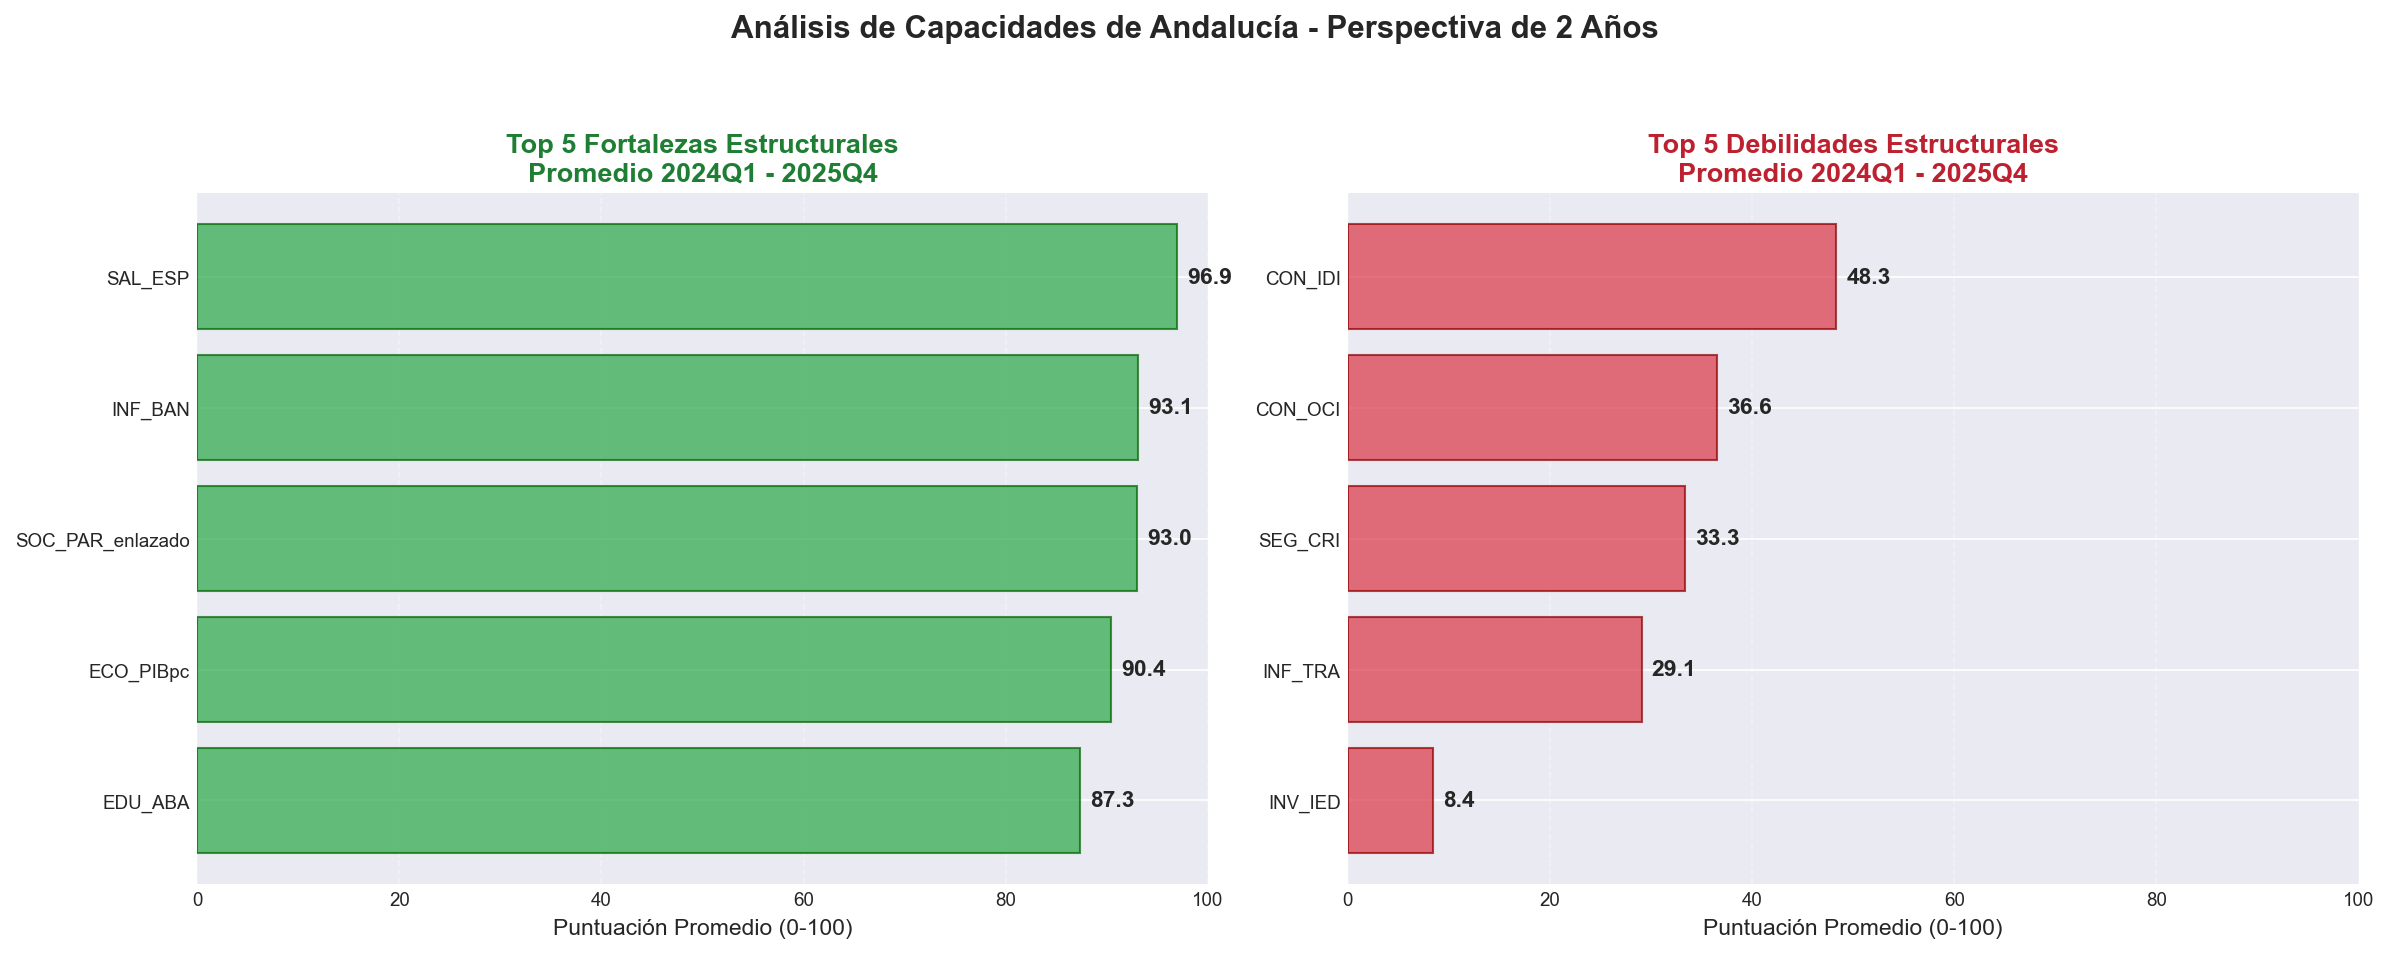
\includegraphics[width=0.85\textwidth]{ipa27_top_bottom_indicadores_2y.png}
    \vfill
    \begin{itemize}
        \item Análisis detallado de la \textbf{variación acumulada} por indicador en el último bienio.
        \item \textbf{Impulsores}: Notable tracción en \textbf{Inversión Extranjera (IED)} y \textbf{Eficiencia en Gobernanza}.
        \item \textbf{Retos Estructurales}: La \textbf{Satisfacción Sanitaria} y la \textbf{Pobreza Relativa (AROPE)} muestran indicadores con mayor margen de mejora en este periodo.
    \end{itemize}
\end{frame}

\begin{frame}{Momentum YoY: ¿Qué empuja el crecimiento?}
    \centering
    
\includegraphics[width=0.7\linewidth]{ipa27_contribuciones_yoy.png}
    \vfill
    \begin{columns}
        \begin{column}{0.6\textwidth}
            \footnotesize
            \textbf{Atribución Logarítmica Exacta}
            \[ \text{Aportación}_d = \frac{\Delta\text{IPA27}}{\ln\text{IPA27}_t - \ln\text{IPA27}_{t-4}} \cdot \frac{1}{3} \cdot \left(\ln D_{d,t} - \ln D_{d,t-4}\right) \]
        \end{column}
        \begin{column}{0.4\textwidth}
            \scriptsize
            \begin{itemize}
                \item Descomposición aditivamente consistente para medias geométricas.
                \item Identifica el peso real de cada dominio en la tasa de variación.
            \end{itemize}
        \end{column}
    \end{columns}
\end{frame}

\begin{frame}{Semáforo de Convergencia: ¿Se cierra la brecha?}
    \begin{columns}
        \begin{column}{0.65\textwidth}
            \centering
            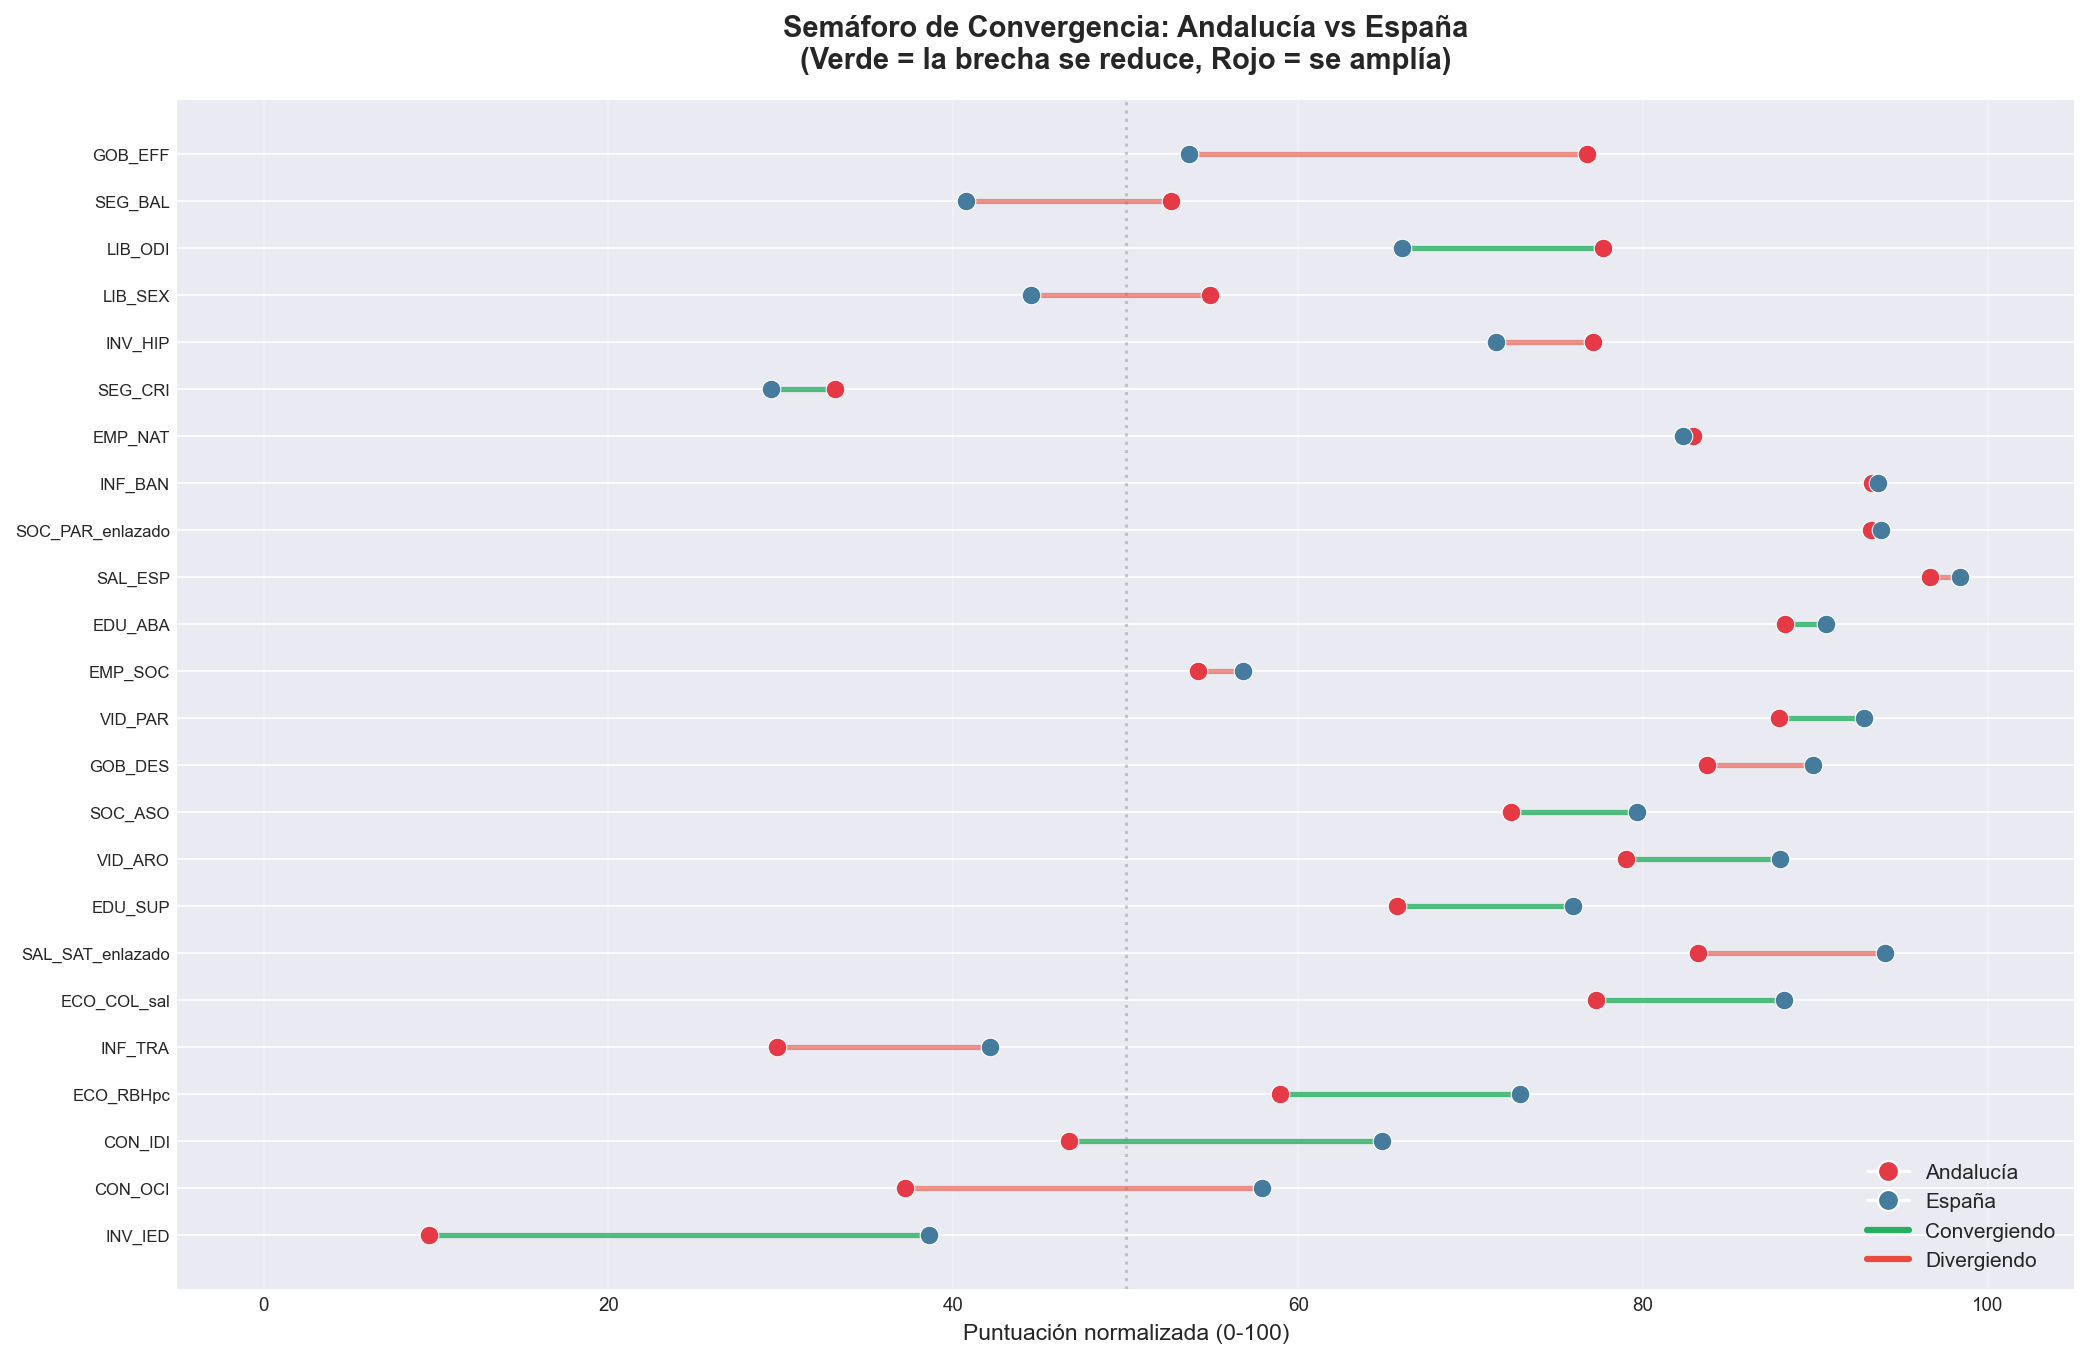
\includegraphics[width=\textwidth]{ipa27_semaforo_convergencia.png}
        \end{column}
        \begin{column}{0.35\textwidth}
            \textbf{Dinámica AND vs ESP}
            \begin{itemize}
                \item \textcolor{brandgreen}{\textbf{Verde (Convergencia)}}: Notable en \textbf{Renta de Hogares}, \textbf{Coste Salarial} e \textbf{Inversión Extranjera}.
                \item \textcolor{red}{\textbf{Rojo (Divergencia)}}: Se observa en \textbf{Satisfacción Sanitaria}, \textbf{Transporte Público} y \textbf{Seguridad}.
                \item Los factores económicos están traccionando la convergencia real, mientras que los sociales presentan desafíos de brecha creciente.
            \end{itemize}
        \end{column}
    \end{columns}
\end{frame}

\begin{frame}{Evolución por Pilares: Heatmap de Puntuaciones}
    \centering
    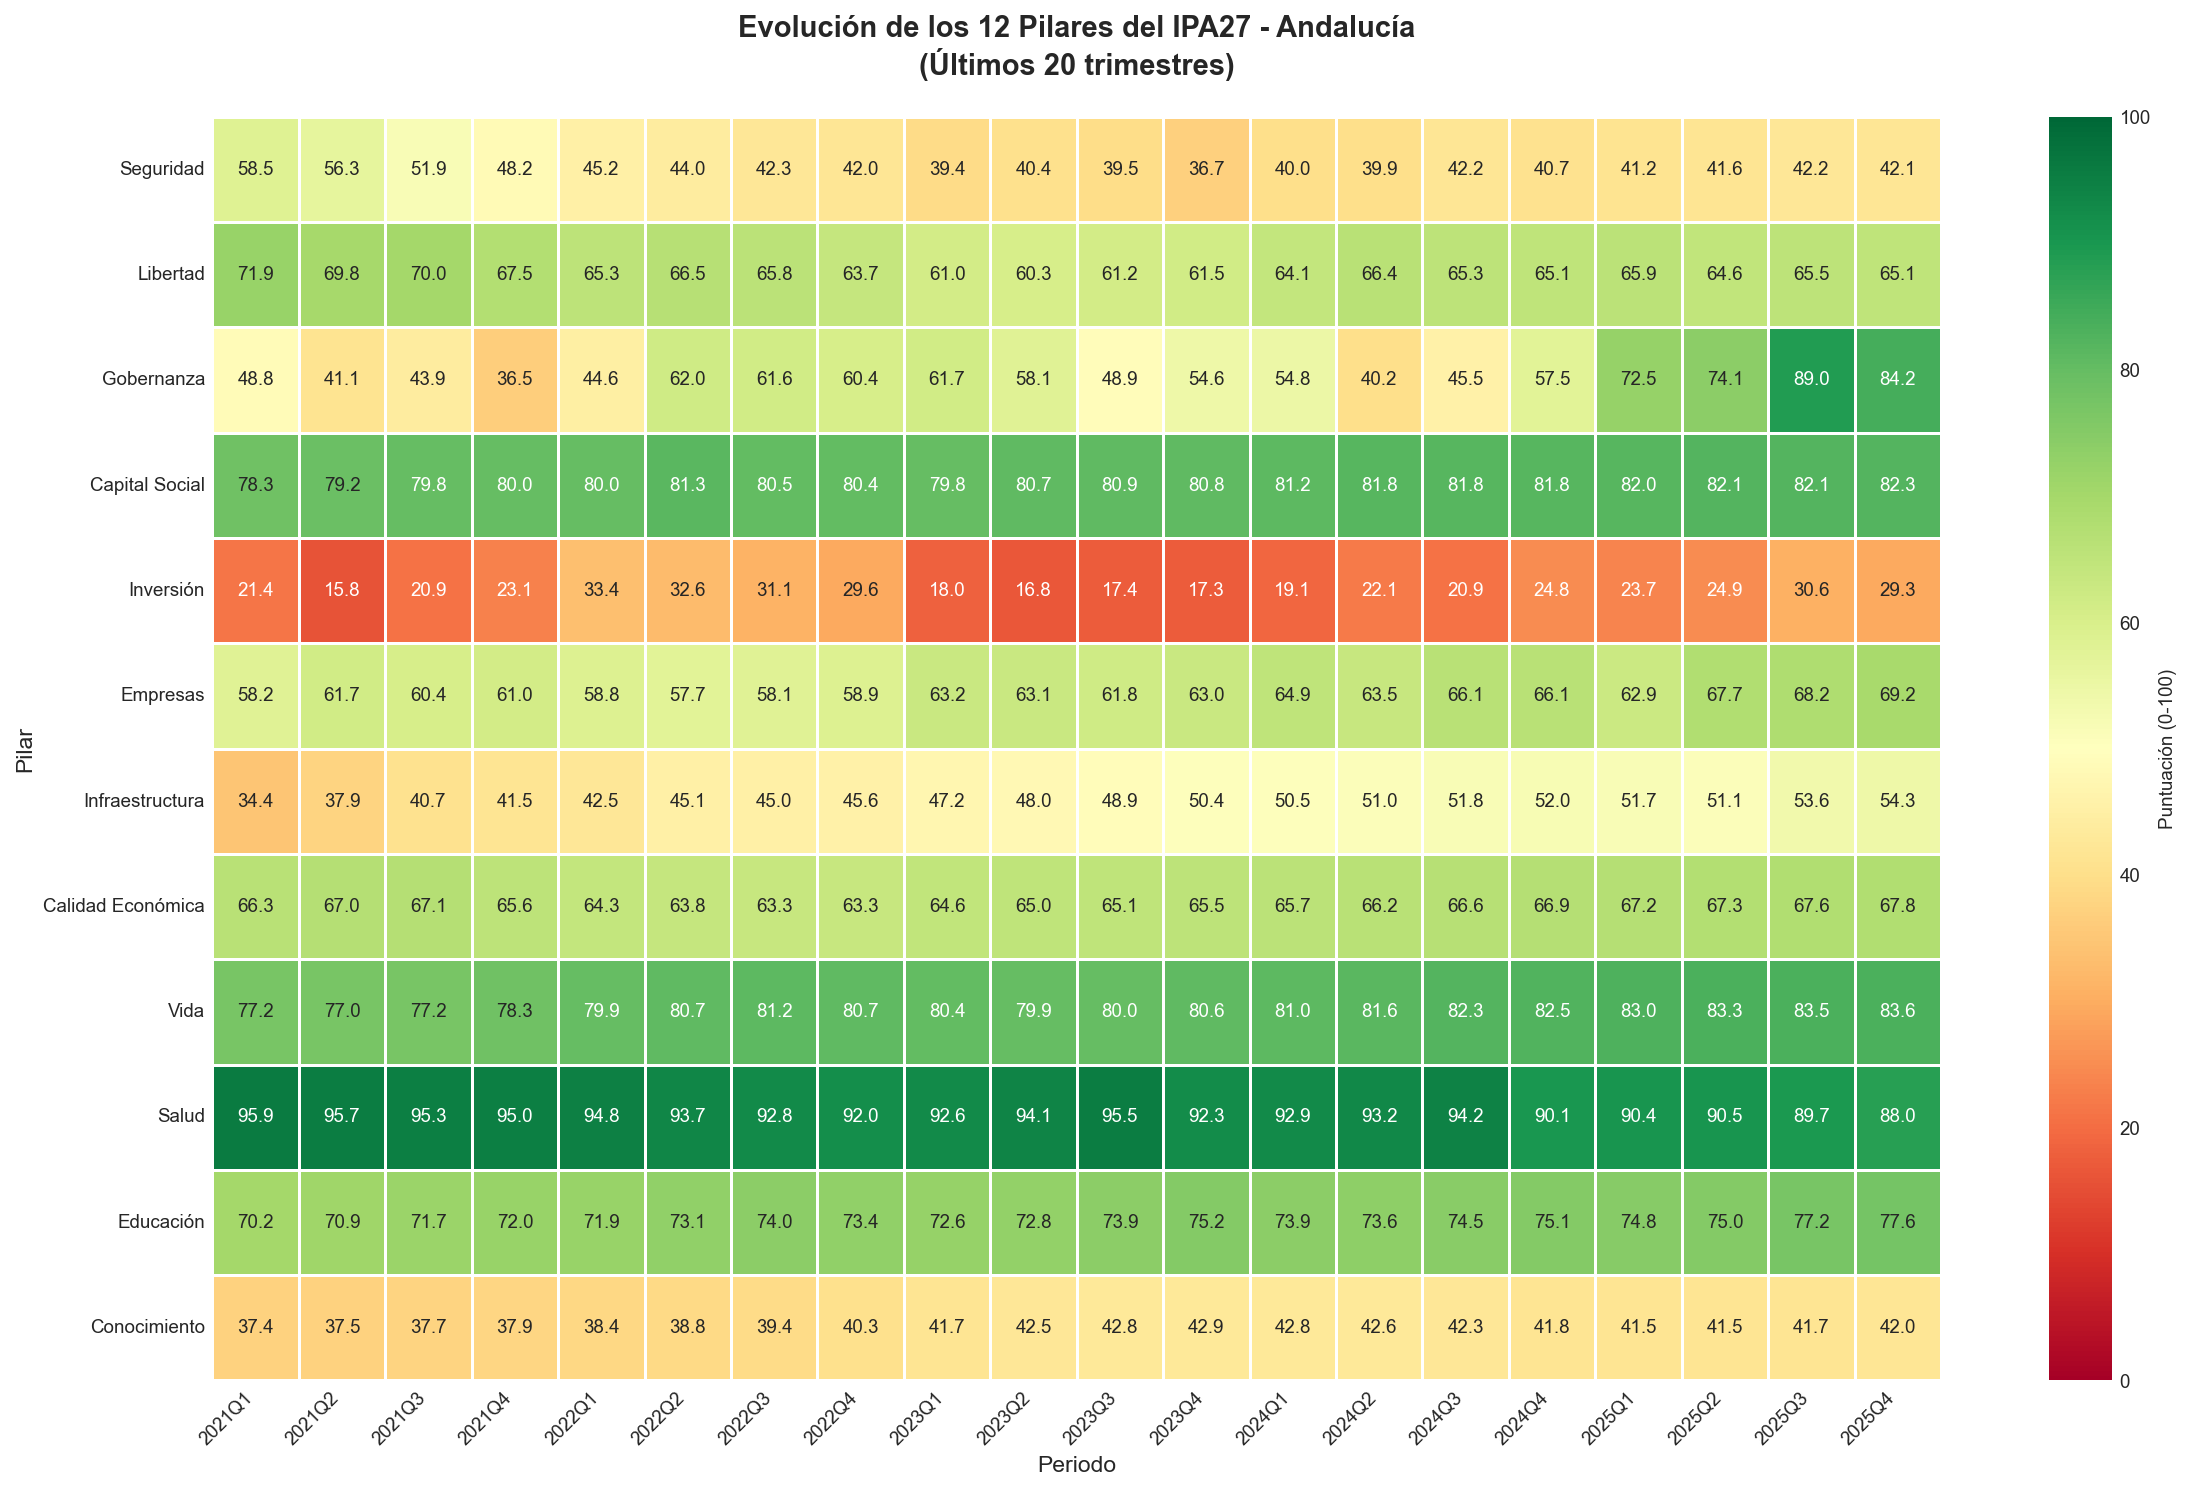
\includegraphics[width=0.8\textwidth]{ipa27_heatmap_pilares.png}
    \vfill
    \begin{itemize}
        \item Visualización de la \textbf{puntuación normalizada (0-100)} para los 12 pilares del índice.
        \item El mapa refleja una \textbf{transición hacia el verde} (mejora sólida) en la mayoría de dimensiones desde 2022.
        \item Pilares como \textbf{Gobernanza} y \textbf{Salud} mantienen niveles de excelencia por encima de los 80 puntos.
    \end{itemize}
\end{frame}

\begin{frame}{Velocidad de Cambio: Momentum de los Pilares}
    \centering
    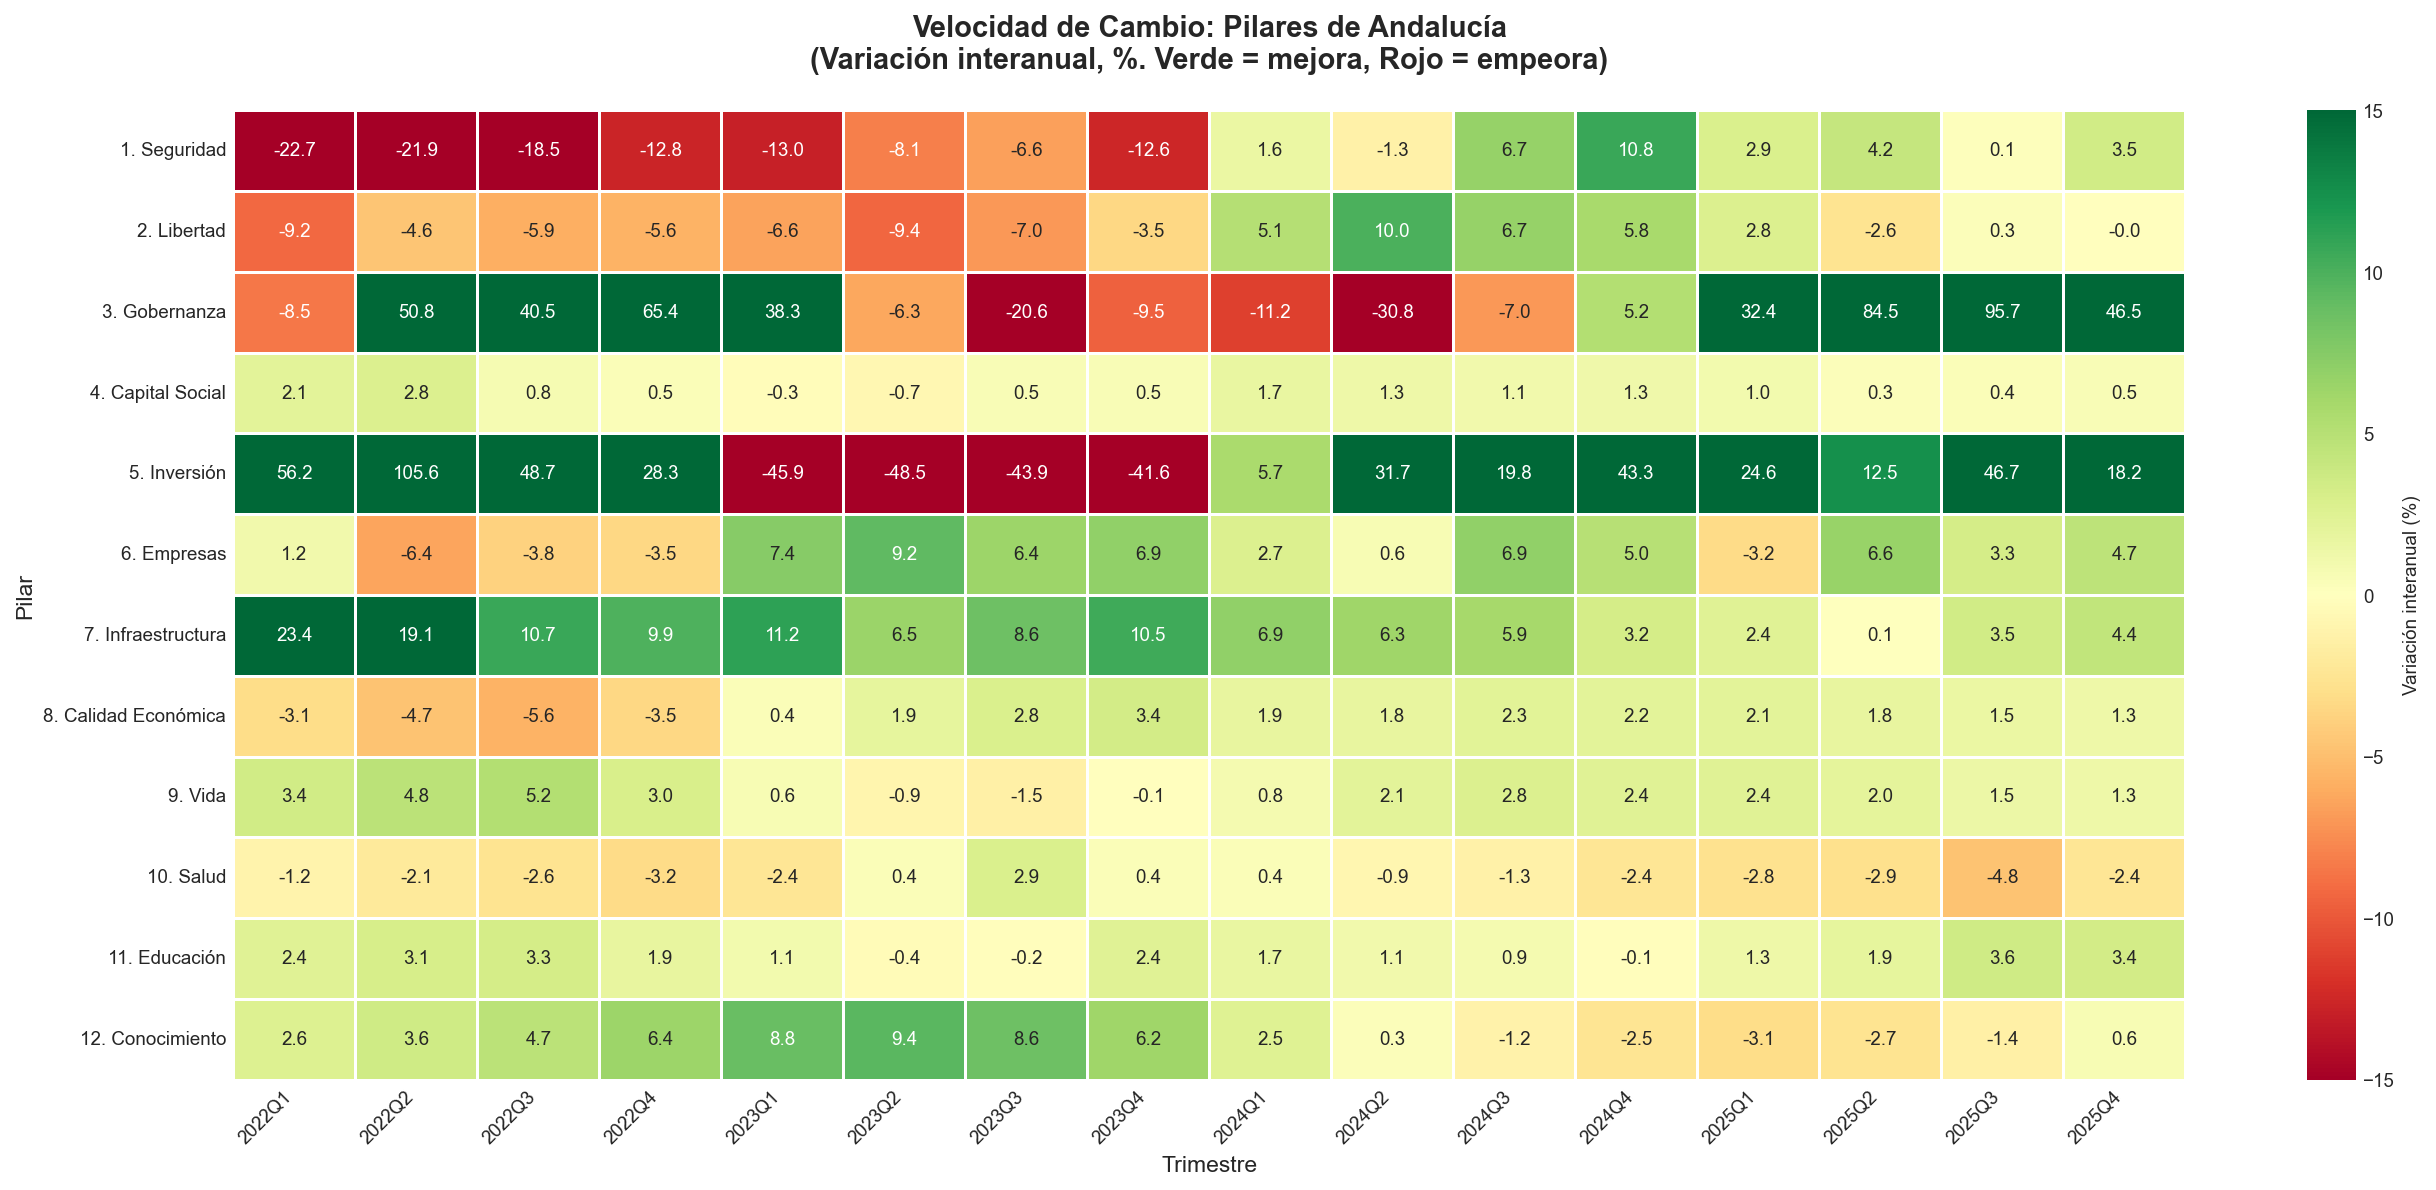
\includegraphics[width=0.85\textwidth]{ipa27_heatmap_velocidad.png}
    \vfill
    \begin{itemize}
        \item Heatmap de \textbf{variaciones interanuales} por pilar (2022-2025).
        \item Periodos de alta aceleración en \textbf{Gobernanza} e \textbf{Inversión} en 2024.
        \item Recuperación sostenida en el pilar de \textbf{Seguridad} tras un inicio de periodo volátil.
    \end{itemize}
\end{frame}

\begin{frame}{Waterfall: Anatomía de la Brecha IPA27}
    \small
    \centering
    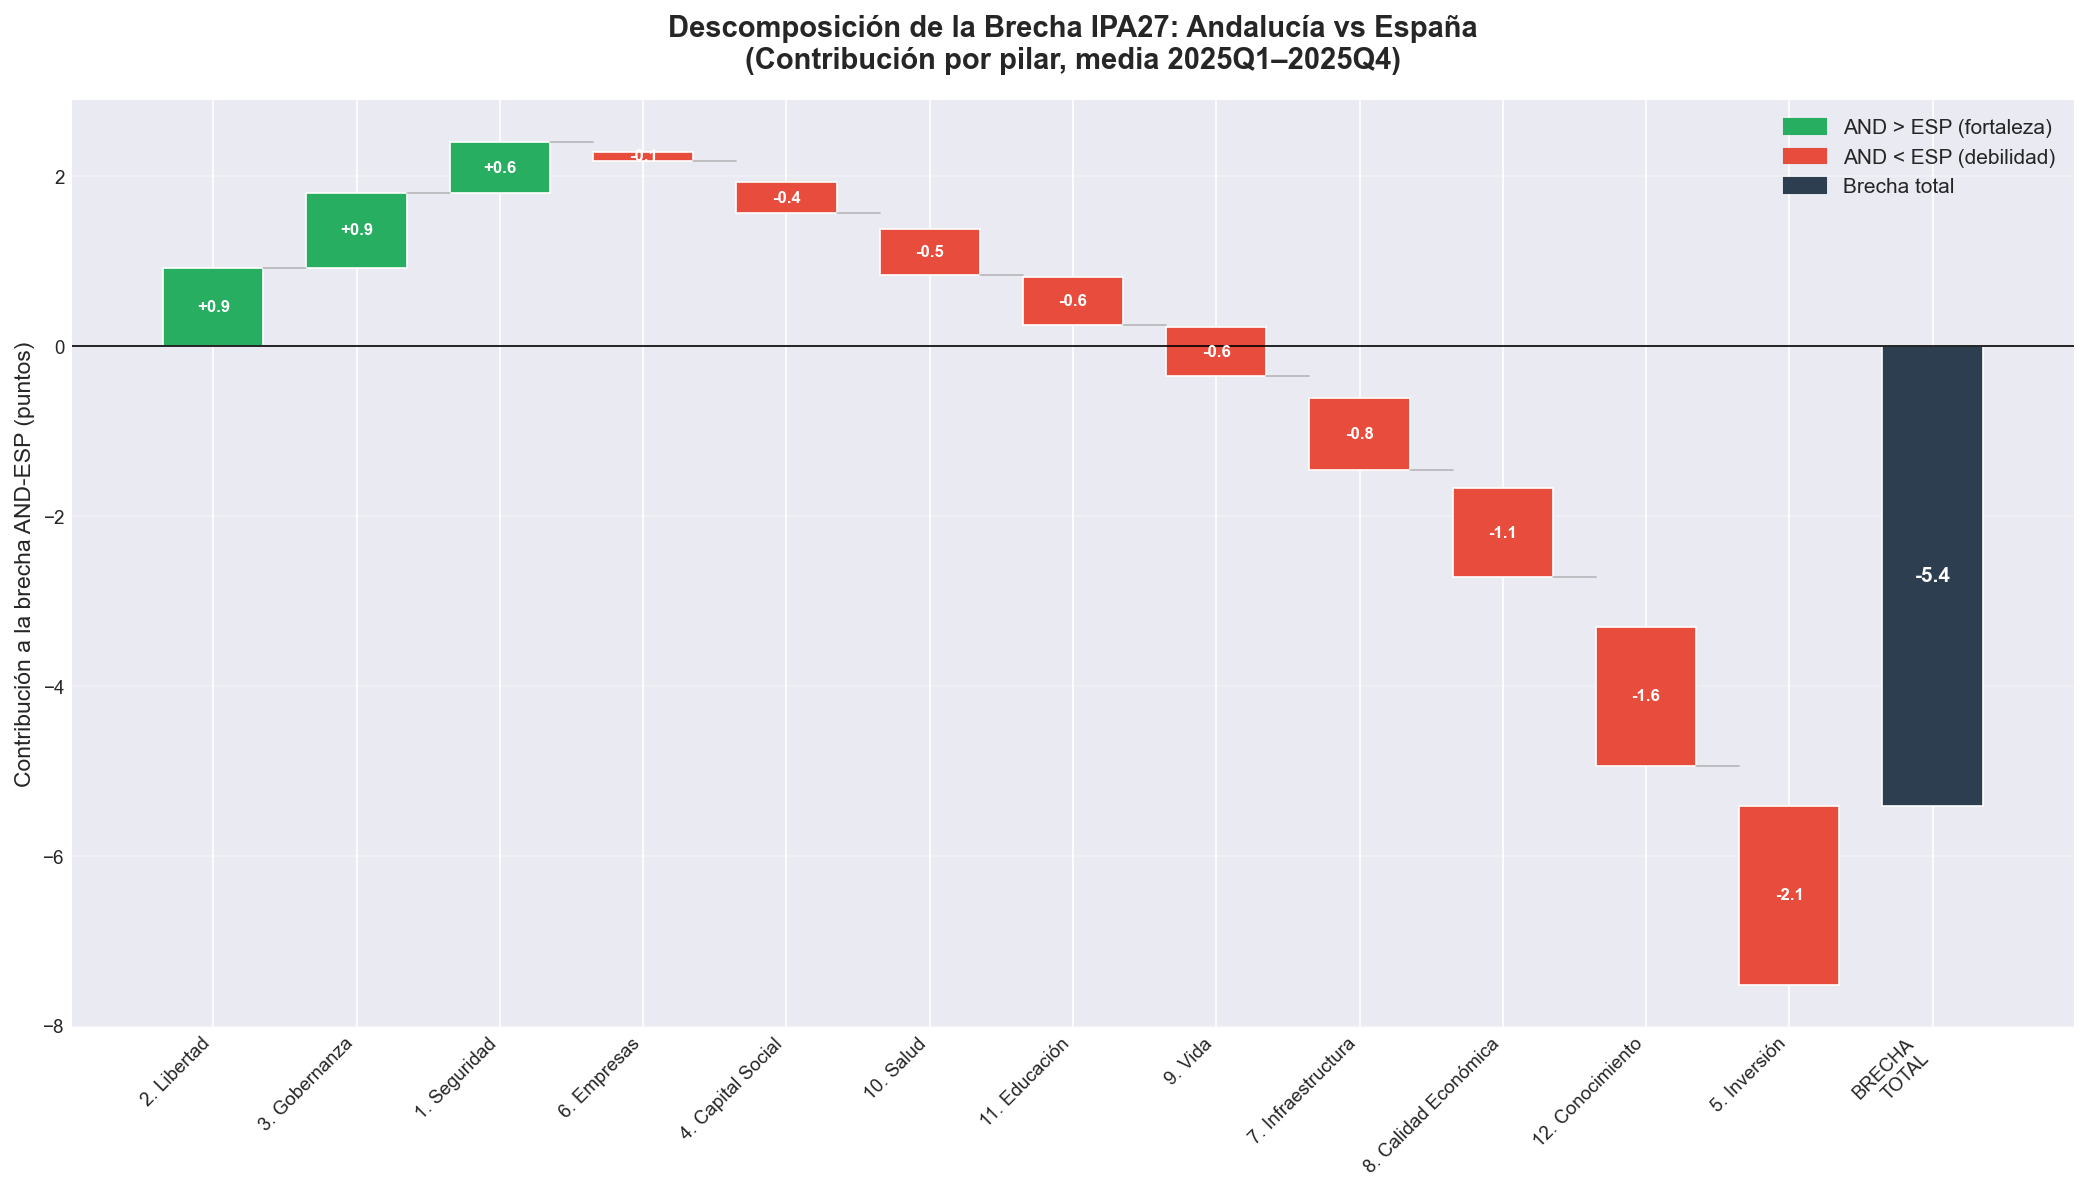
\includegraphics[width=0.7\textwidth]{ipa27_waterfall_brecha.png}
    \vfill
    \begin{itemize}
        \item \textbf{Brecha neta de -5.4 puntos} frente a la media nacional (2025Q4).
        \item \textbf{Fortalezas}: Libertad (+0.9), Gobernanza (+0.9) y Seguridad (+0.6).
        \item \textbf{Debilidades estructurales}: Inversión (-2.1), Conocimiento (-1.6) y Calidad Económica (-1.1).
    \end{itemize}
\end{frame}

\begin{frame}{Mapa de Posicionamiento y Trayectorias (2019-2025)}
    \begin{columns}
        \begin{column}{0.6\textwidth}
            \centering
            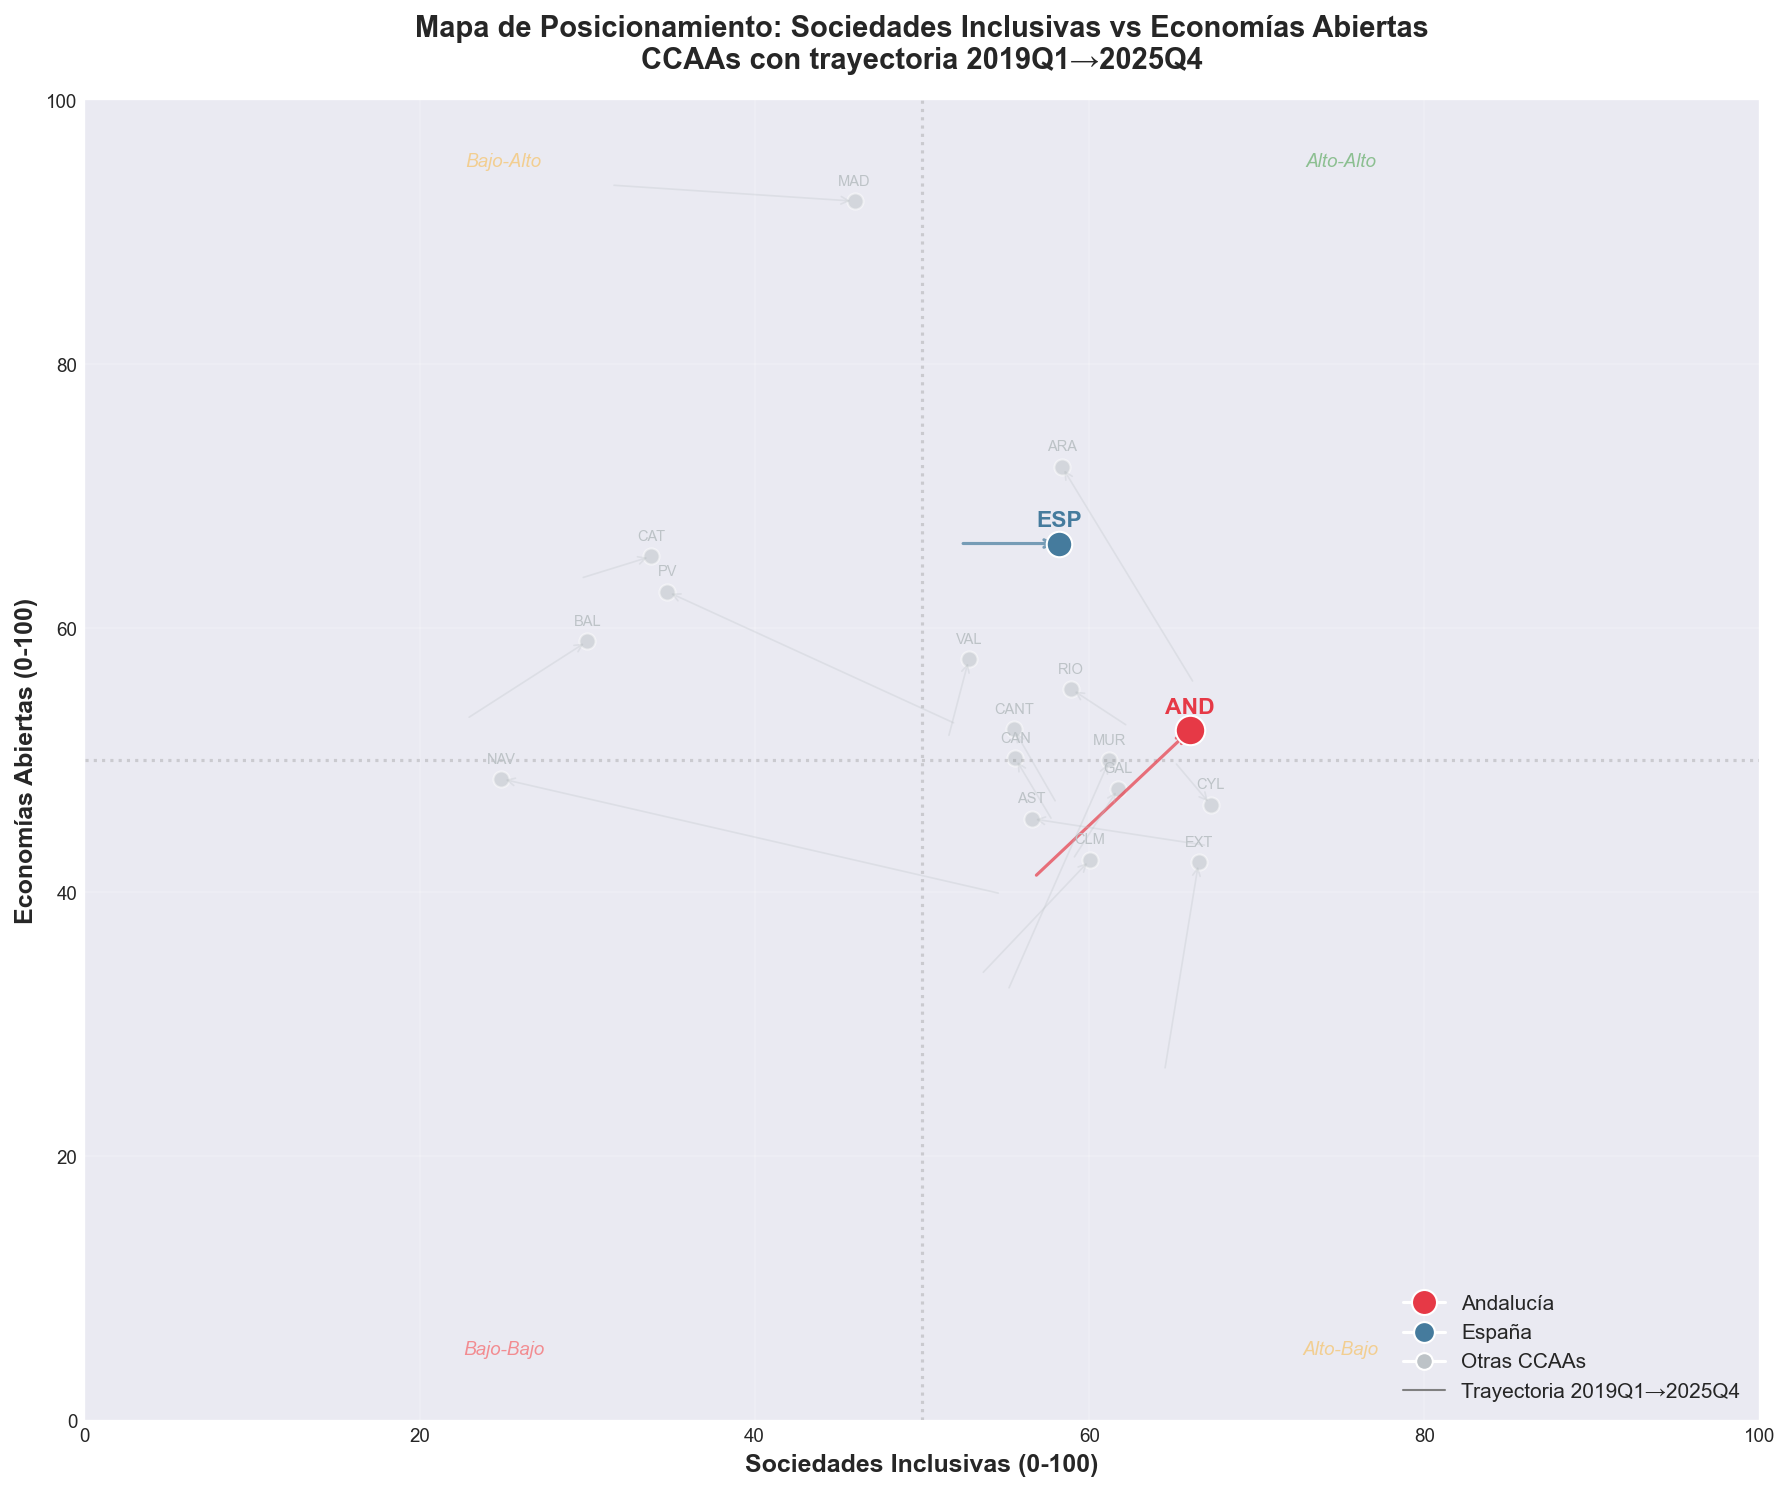
\includegraphics[width=\textwidth]{ipa27_scatter_gapminder.png}
        \end{column}
        \begin{column}{0.4\textwidth}
            \textbf{Análisis de Desplazamiento}
            \begin{itemize}
                \item Cruce: \textbf{Sociedades Inclusivas} vs \textbf{Economías Abiertas}.
                \item Las flechas indican el vector desde 2019Q1 hasta 2025Q4.
                \item Andalucía muestra una \textbf{mejora sólida y equilibrada} en ambos ejes, desplazándose hacia el cuadrante de mayor prosperidad relativa.
            \end{itemize}
        \end{column}
    \end{columns}
\end{frame}

\begin{frame}{Posición de Andalucía en la Distribución Regional}
    \centering
    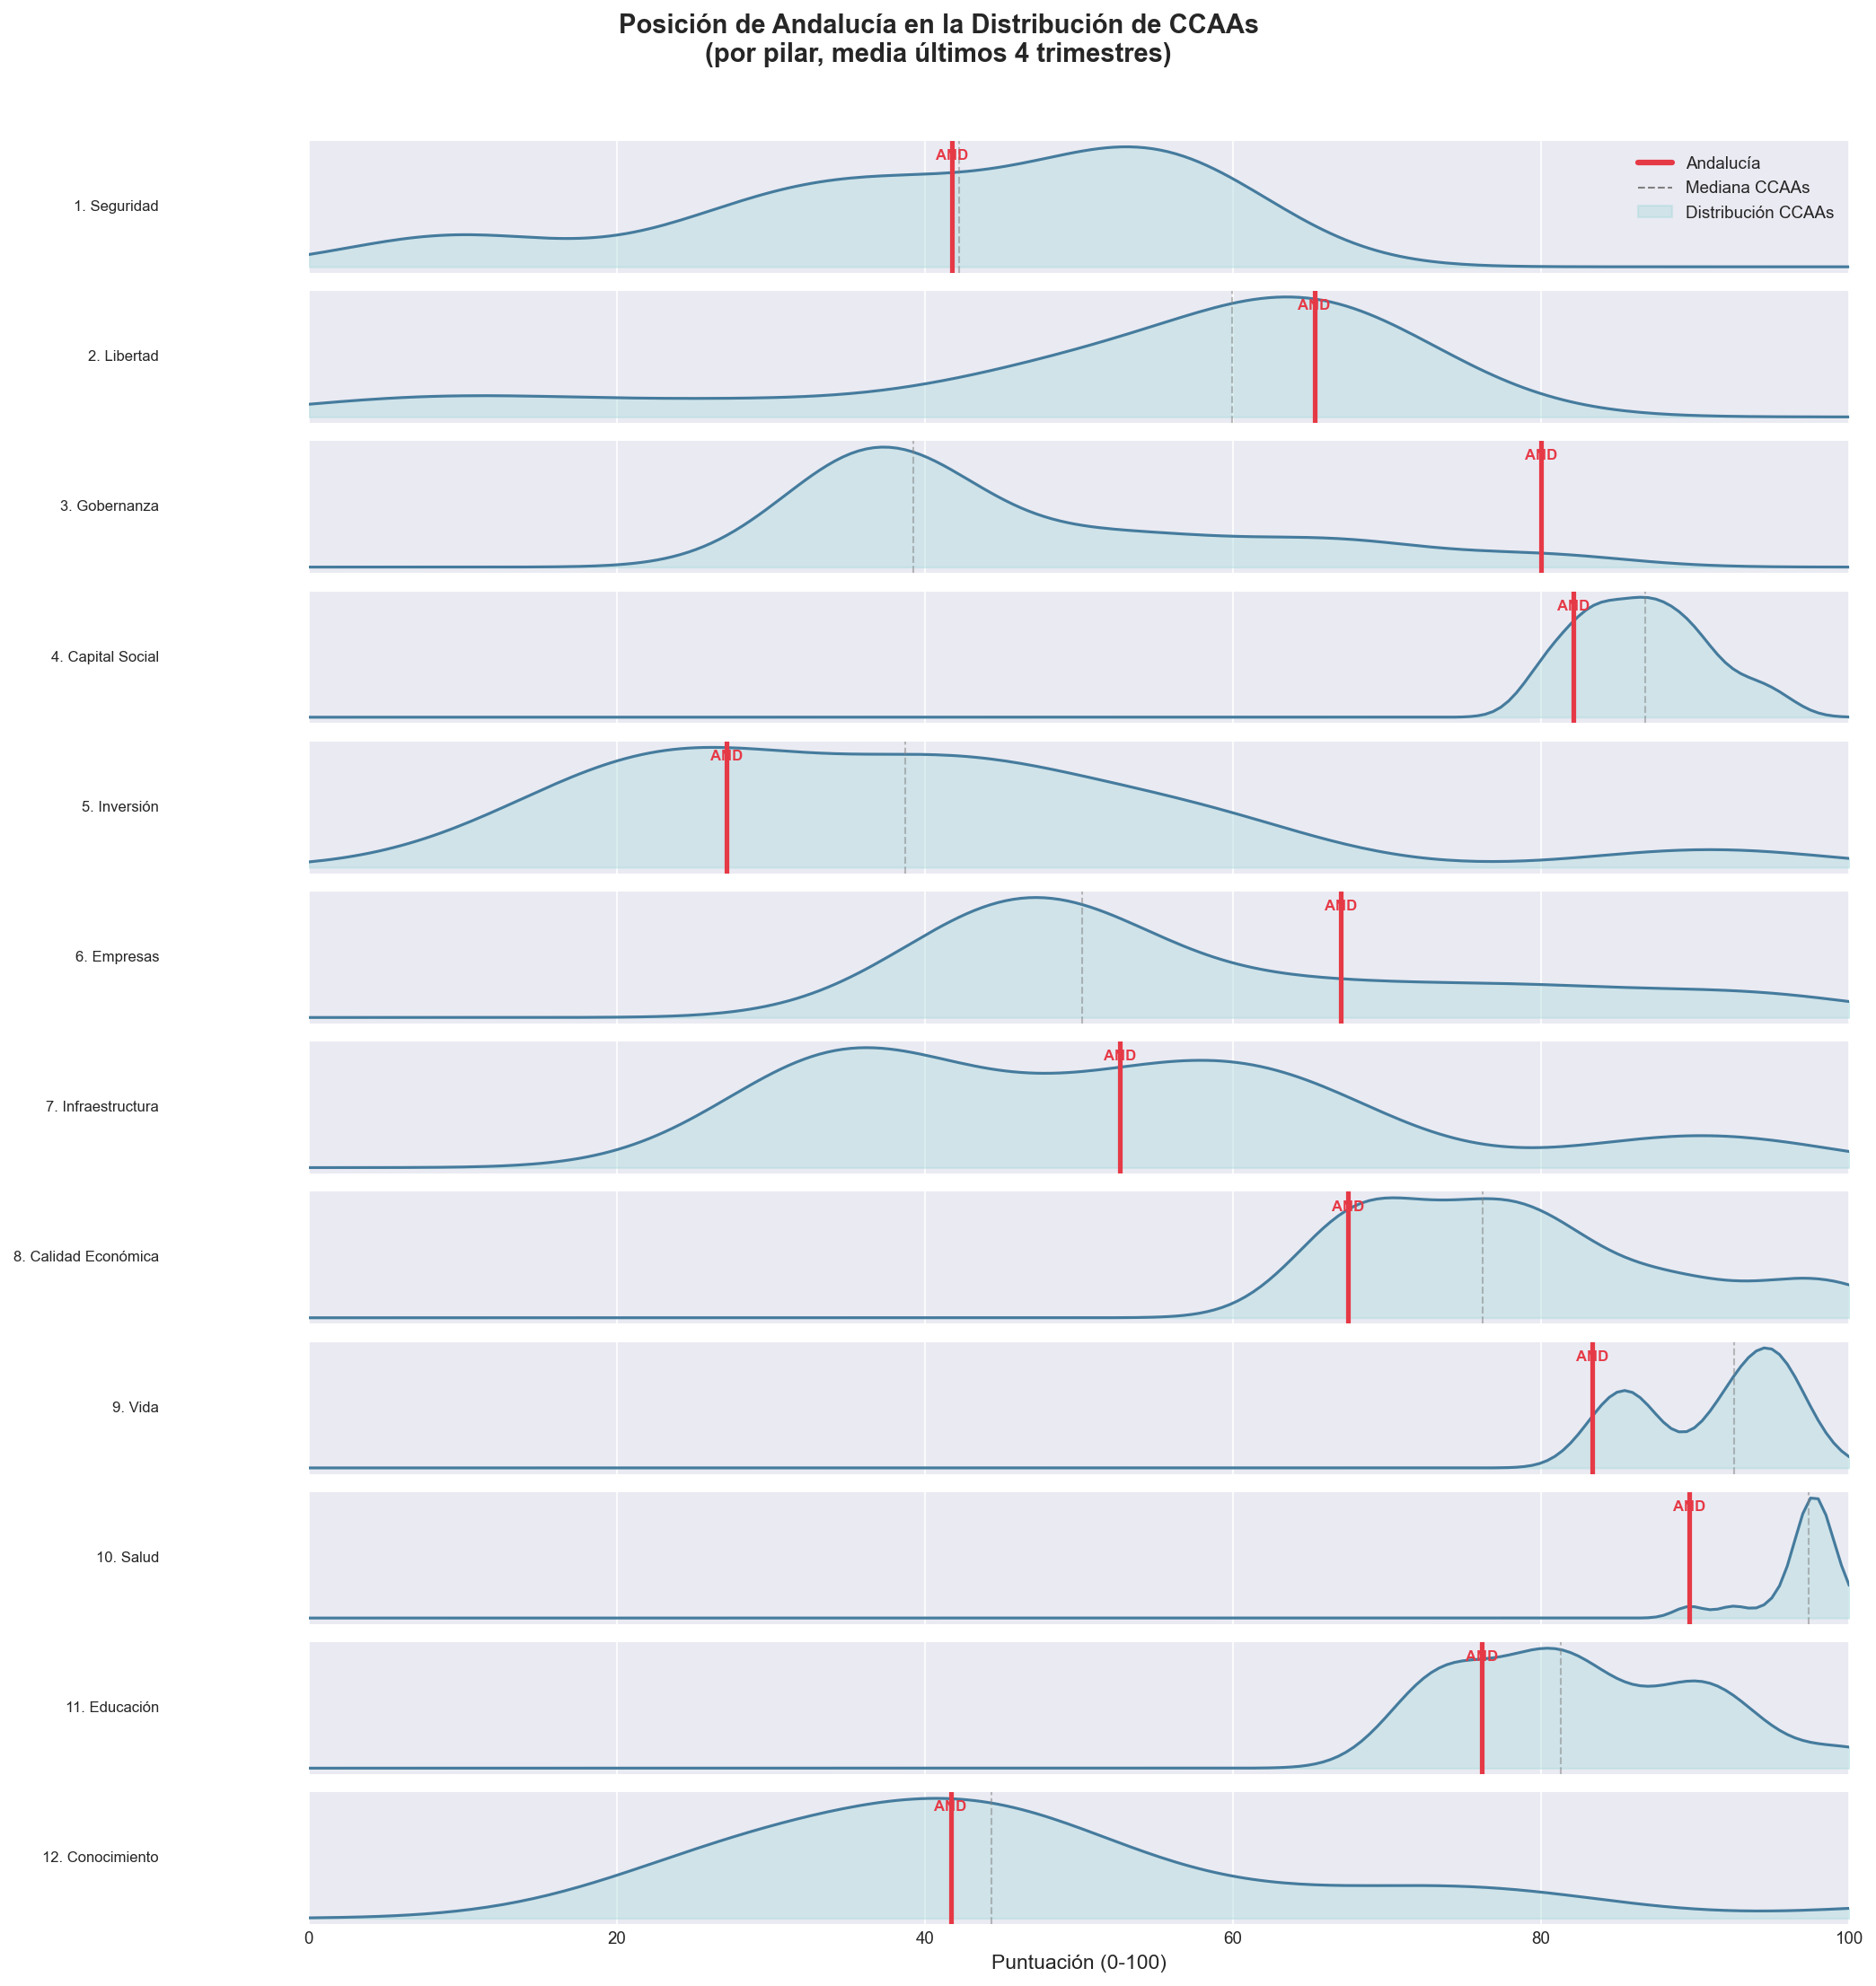
\includegraphics[width=0.7\linewidth]{ipa27_ridgeline_pilares.png}
    \vfill
    \begin{itemize}
        \item \textbf{Ridgeline Analysis}: Distribución de las 17 CCAA para cada pilar.
        \item Andalucía destaca positivamente (sobre la mediana) en \textbf{Libertad} y \textbf{Gobernanza}.
        \item Se sitúa cerca de la mediana en \textbf{Seguridad} y \textbf{Salud}.
    \end{itemize}
\end{frame}

% --- 5. AUDITORÍA Y CONCLUSIÓN ---
\section{Auditoría}

{
\setbeamercolor{background canvas}{bg=brandgreen}
\begin{frame}[plain]
    \centering
    \vfill
    {\Huge\bfseries\color{white} V. AUDITORÍA}\\[0.6cm]
    {\color{white}\rule{6cm}{2.5pt}}\\[1.5cm]
    
\includegraphics[width=2.5cm]{logo_fa27_white.png}
    \vfill
\end{frame}
}

\begin{frame}{Sistema de Auditoría y Trazabilidad}
    \begin{columns}
        \begin{column}{0.6\textwidth}
            \textbf{Garantía de Calidad (Quality Assurance)}
            \begin{itemize}
                \item \textbf{Capa 1}: Registro de orígenes de datos brutos.
                \item \textbf{Capa 2}: Excel de Auditoría de Normalización (vínculo Dato $\rightarrow$ Techo $\rightarrow$ Score).
                \item \textbf{Capa 3}: Fichas PDF de Indicadores (24 gráficos de evolución individual).
            \end{itemize}
        \end{column}
        \begin{column}{0.4\textwidth}
            \begin{block}{Rigor Científico}
                El IPA27 cumple con el estándar de replicabilidad: cualquier auditor puede reconstruir el índice desde el dato bruto oficial.
            \end{block}
        \end{column}
    \end{columns}
\end{frame}

\begin{frame}{Conclusiones y Futuro del IPA27}
    \begin{itemize}
        \item \textbf{Métrica de Estado}: No es solo un dato económico, es un diagnóstico de la salud social de la región.
        \item \textbf{Herramienta de Política Pública}: Ayuda a priorizar inversiones en los pilares con mayor rezago.
        \item \textbf{Actualización Continua}: Pipeline robusto que permite reportar resultados apenas semanas después de las fuentes oficiales.
    \end{itemize}
    \vspace{0.8cm}
    \centering
    {\Large \textbf{\textcolor{brandgreen}{Hacia una Andalucía más Próspera y Equitativa}}}
\end{frame}

% --- Slide Final ---
{
\setbeamertemplate{footline}{} 
\begin{frame}[plain]
    \centering
    \vspace{2cm}
    {\huge \textbf{\textcolor{brandgreen}{Gracias por su atención}}}
    
    \vspace{1cm}
    \begin{tikzpicture}
        \fill[brandgreen] (-4,0) rectangle (4, 0.05);
    \end{tikzpicture}
    
    \vspace{1cm}
    \footnotesize
    Persona de contacto: \textit{mhidper@upo.es}\\
    Repositorio de Datos: \texttt{metodologia/01\_IPA27\_General}
\end{frame}
}

\end{document}
